\caulc
\begin{ex}%[TDMZZ18]%[Nguyễn Tấn Linh]%[1D6N2-1]
	Giá trị của $\log(10\mathrm{e})$ bằng
	\choice
	{$1$}
	{$1+\ln 10$}
	{\True $1+\dfrac{1}{\ln 10}$}
	{$2$}
	\loigiai{
		Ta có $\log(10\mathrm{e}) = \log 10 + \log \mathrm{e} = 1 + \dfrac{\ln \mathrm{e}}{\ln 10} = 1 + \dfrac{1}{\ln 10}$.
	}
\end{ex}

\begin{ex}%[TDMZZ18]%[Nguyễn Tấn Linh]%[1D6N3-1]
	Tập giá trị của hàm số $y=\mathrm{e}^x$ là
	\choice
	{\True $(0;+\infty)$}
	{$\mathbb{R}$}
	{$\mathbb{R}\setminus\{0\}$}
	{$(\mathrm{e};+\infty)$}
	\loigiai{
		Hàm số mũ $y=a^x$ (với $0<a\neq 1$) có tập xác định là $\mathbb{R}$ và tập giá trị là $(0;+\infty)$.\\
		Do đó, tập giá trị của hàm số $y=\mathrm{e}^x$ là $(0;+\infty)$.
	}
\end{ex}

\begin{ex}%[TDMZZ18]%[Nguyễn Tấn Linh]%[1D3H2-5]
	Giá trị của $\lim\limits_{x\to -\infty}\left(\sqrt{x^2+4x}+x\right)$ bằng
	\choice
	{$2$}
	{\True $-2$}
	{$1$}
	{$0$}
	\loigiai{
		Ta có
		\allowdisplaybreaks
		\begin{eqnarray*}
			\lim\limits_{x\to -\infty}\left(\sqrt{x^2+4x}+x\right)
			&=& \lim\limits_{x\to -\infty}\dfrac{x^2+4x-x^2}{\sqrt{x^2+4x}-x}\\
			&=& \lim\limits_{x\to -\infty}\dfrac{4x}{|x|\sqrt{1+\dfrac{4}{x}}-x}\\
			&=& \lim\limits_{x\to -\infty}\dfrac{4x}{-x\sqrt{1+\dfrac{4}{x}}-x}\\
			&=& \lim\limits_{x\to -\infty}\dfrac{4}{-\sqrt{1+\dfrac{4}{x}}-1}\\
			&=& \dfrac{4}{-1-1}=-2.
		\end{eqnarray*}
	}
\end{ex}

\begin{ex}%[TDMZZ18]%[Nguyễn Tấn Linh]%[1H8H1-2]
	\immini{Cho hình chóp $S. ABC$ có $\triangle ABC$ vuông tại $B$, $SA\perp (ABC)$. Đáp án cho nhận xét \textbf{sai} là
		\choice
		{$BC\perp SB$}
		{$SA\perp BC$}
		{$SA\perp AC$}
		{\True $AB\perp SC$}
	}
	{\begin{tikzpicture}[line join=round, line cap=round, >=stealth, font=\footnotesize, scale=0.8]
			\coordinate (A) at (0,0);
			\coordinate (C) at (5,0);
			\coordinate (B) at (1.5,-2);
			\coordinate (S) at (0,4);
			\draw[dashed, thick] (A) -- (C);
			\draw[thick] (S) -- (A) -- (B) -- (C) -- (S);
			\draw[thick] (S) -- (B);
			\coordinate (B1) at ($(B)!0.4cm!(A)$);
			\coordinate (B2) at ($(B)!0.4cm!(C)$);
			\coordinate (B3) at ($(B1)+(B2)-(B)$);
			\draw (B1) -- (B3) -- (B2);
			\coordinate (A1) at ($(A)!0.4cm!(B)$);
			\coordinate (A2) at ($(A)!0.4cm!(S)$);
			\coordinate (A3) at ($(A1)+(A2)-(A)$);
			\draw (A1) -- (A3) -- (A2);
			\coordinate (A4) at ($(A)!0.4cm!(C)$);
			\coordinate (A5) at ($(A2)+(A4)-(A)$);
			\draw[dashed] (A4) -- (A5) -- (A2);
			\node[left] at (A) {$A$};
			\node[right] at (C) {$C$};
			\node[below] at (B) {$B$};
			\node[above] at (S) {$S$};
		\end{tikzpicture}
	}
	\loigiai{
		\begin{itemize}
			\item Vì $SA\perp (ABC)$ nên $SA\perp BC$ và $SA\perp AC$. Suy ra các nhận xét $SA\perp BC$ và $SA\perp AC$ đúng.
			\item Ta có $\heva{&BC\perp AB\\ &BC\perp SA}\Rightarrow BC\perp (SAB)\Rightarrow BC\perp SB$. Suy ra nhận xét $BC\perp SB$ đúng.
			\item Nếu $AB\perp SC$, kết hợp với $AB\perp SA$, ta suy ra $AB\perp (SAC)\Rightarrow AB\perp AC$. Điều này mâu thuẫn với giả thiết tam giác $ABC$ vuông tại $B$. Do đó nhận xét $AB\perp SC$ là sai.
		\end{itemize}
	}
\end{ex}

\begin{ex}%[TDMZZ18]%[Nguyễn Tấn Linh]%[2D1N2-2]
	\immini[thm]{Cho hàm số $y=f(x)$ có đồ thị như hình vẽ, $f(x)$ đạt cực đại tại điểm
		\choice
		{\True $x=1$}
		{$y=3$}
		{$x=-3$}
		{$x=3$}
	}
	{
		\begin{tikzpicture}[line join=round, line cap=round, >=stealth, font=\footnotesize, scale=0.8]
			\draw[->] (-4.5,0)--(5.5,0) node[below]{$x$};
			\draw[->] (0,-4.5)--(0,4) node[right]{$y$};
			\fill (0,0) circle (1.5pt) node[below left]{$O$};
			\draw[dashed] (-3,0) node[above]{$-3$}--(-3,-4)--(0,-4) node[right]{$-4$};
			\draw[dashed] (1,0) node[below right]{$1$}--(1,3)--(0,3) node[left]{$3$};
			\draw[dashed] (4,0) node[above]{$4$}--(4,-2)--(0,-2) node[left]{$-2$};
			\fill (-3,-4) circle (1.5pt);
			\fill (1,3) circle (1.5pt);
			\fill (4,-2) circle (1.5pt);
			\draw[thick, blue] (-4,1)--(-3,-4)--(1,3)--(4,-2)--(5,2);
			\node at (2,3.5) {$f(x)$};
		\end{tikzpicture}
	}
	\loigiai{
		Dựa vào đồ thị, ta thấy điểm cực đại của đồ thị hàm số là $(1;3)$.\\
		Vậy hàm số đạt cực đại tại điểm $x=1$.
	}
\end{ex}

\begin{ex}%[TDMZZ18]%[Nguyễn Tấn Linh]%[2H5N1-2]
	Trong không gian với hệ trục tọa độ $Oxyz$, cho mặt phẳng $(P)\colon -x+2y+z+6=0$. Một vectơ pháp tuyến của mặt phẳng $(P)$ là
	\choice
	{\True $(-1;2;1)$}
	{$(6;-1;2)$}
	{$(3;-1;0)$}
	{$(0;1;-3)$}
	\loigiai{
		Mặt phẳng $(P)\colon -x+2y+z+6=0$ có một vectơ pháp tuyến là $\overrightarrow{n}_P=(-1;2;1)$.
	}
\end{ex}

\begin{ex}%[TDMZZ18]%[Nguyễn Tấn Linh]%[2D4N3-1]
	Cho hình phẳng $(H)$ giới hạn bởi các đường $y=x^2-2x$, $Ox$, $x=a$, $x=b$ ($a<b$). Diện tích hình phẳng của $(H)$ là
	\choice
	{$S=\displaystyle\int\limits_{0}^{2}\left|x^2-2x\right|\mathrm{\,d}x$}
	{\True $S=\displaystyle\int\limits_{a}^{b}\left|x^2-2x\right|\mathrm{\,d}x$}
	{$S=\displaystyle\int\limits_{a}^{b}(x^2-2x)\mathrm{\,d}x$}
	{$S=\displaystyle\int\limits_{0}^{2}(x^2-2x)\mathrm{\,d}x$}
	\loigiai{
		Diện tích hình phẳng giới hạn bởi đồ thị hàm số $y=f(x)$, trục hoành $y=0$ và hai đường thẳng $x=a$, $x=b$ ($a<b$) được tính bởi công thức $S=\displaystyle\int\limits_{a}^{b}|f(x)|\mathrm{\,d}x$.\\
		Do đó, diện tích hình phẳng của $(H)$ là $S=\displaystyle\int\limits_{a}^{b}\left|x^2-2x\right|\mathrm{\,d}x$.
	}
\end{ex}

\begin{ex}%[TDMZZ18]%[Nguyễn Tấn Linh]%[2D1H4-1]
	Số đường tiệm cận của đồ thị hàm số $y=\dfrac{x+1}{x^2-4}$ là
	\choice
	{$1$}
	{$2$}
	{$0$}
	{\True $3$}
	\loigiai{
		Tập xác định $\mathscr{D}=\mathbb{R}\setminus\{-2;2\}$.\\
		Ta có $\lim\limits_{x\to \pm\infty}y=\lim\limits_{x\to \pm\infty}\dfrac{x+1}{x^2-4}=0 \Rightarrow$ đồ thị hàm số có $1$ đường tiệm cận ngang là $y=0$.\\
		Mặt khác, $\lim\limits_{x\to 2^+}y=\lim\limits_{x\to 2^+}\dfrac{x+1}{x^2-4}=+\infty$ và $\lim\limits_{x\to (-2)^+}y=\lim\limits_{x\to (-2)^+}\dfrac{x+1}{x^2-4}=+\infty \Rightarrow$ đồ thị hàm số có $2$ đường tiệm cận đứng là $x=2$ và $x=-2$.\\
		Vậy đồ thị hàm số có tổng cộng $3$ đường tiệm cận.
	}
\end{ex}

\begin{ex}%[TDMZZ18]%[Nguyễn Tấn Linh]%[2D4N1-4]
	Họ nguyên hàm của hàm số $\left(\mathrm{e}^x-1\right) \left(\mathrm{e}^{-x}+1\right)$ tương ứng là
	\choice
	{$\mathrm{e}^x-\mathrm{e}^{-x}+C$}
	{$2\mathrm{e}^x+C$}
	{$\mathrm{e}^{2x}+\mathrm{e}^{-2x}+C$}
	{\True $\mathrm{e}^x+\mathrm{e}^{-x}+C$}
	\loigiai{
		Ta có $\left(\mathrm{e}^x-1\right) \left(\mathrm{e}^{-x}+1\right) = 1+\mathrm{e}^x-\mathrm{e}^{-x}-1 = \mathrm{e}^x-\mathrm{e}^{-x}$.\\
		Họ nguyên hàm của hàm số là
		\[ \displaystyle\int \left(\mathrm{e}^x-\mathrm{e}^{-x}\right)\mathrm{\,d}x = \mathrm{e}^x+\mathrm{e}^{-x}+C. \]
	}
\end{ex}

\begin{ex}%[TDMZZ18]%[Nguyễn Tấn Linh]%[2H2H1-2]
	Cho hình chóp $S. ABC$ có $G$ là trọng tâm của $\triangle ABC$. Đáp án cho nhận xét \textbf{sai} là
	\choice
	{$\overrightarrow{GA}+\overrightarrow{GB}+\overrightarrow{GC}=\overrightarrow{0}$}
	{$\overrightarrow{SA}+\overrightarrow{SB}+\overrightarrow{SC}=3\overrightarrow{SG}$}
	{\True $\overrightarrow{SA}+\overrightarrow{SB}-\overrightarrow{CS}=4\overrightarrow{SG}$}
	{$\overrightarrow{GA}+\overrightarrow{GB}-\overrightarrow{GC}=2\overrightarrow{CG}$}
	\loigiai{
		Vì $G$ là trọng tâm tam giác $ABC$ nên ta có:
		\begin{itemize}
			\item $\overrightarrow{GA}+\overrightarrow{GB}+\overrightarrow{GC}=\overrightarrow{0}$. Suy ra nhận xét $\overrightarrow{GA}+\overrightarrow{GB}+\overrightarrow{GC}=\overrightarrow{0}$ đúng.
			\item Với điểm $S$ bất kỳ, ta luôn có $\overrightarrow{SA}+\overrightarrow{SB}+\overrightarrow{SC}=3\overrightarrow{SG}$. Suy ra nhận xét $\overrightarrow{SA}+\overrightarrow{SB}+\overrightarrow{SC}=3\overrightarrow{SG}$ đúng.
			\item Xét $\overrightarrow{GA}+\overrightarrow{GB}-\overrightarrow{GC} = (\overrightarrow{GA}+\overrightarrow{GB}+\overrightarrow{GC}) - 2\overrightarrow{GC} = \overrightarrow{0} - 2\overrightarrow{GC} = 2\overrightarrow{CG}$. Suy ra nhận xét $\overrightarrow{GA}+\overrightarrow{GB}-\overrightarrow{GC}=2\overrightarrow{CG}$ đúng.
			\item Ta có $\overrightarrow{SA}+\overrightarrow{SB}-\overrightarrow{CS} = \overrightarrow{SA}+\overrightarrow{SB}+\overrightarrow{SC} = 3\overrightarrow{SG}$. Do đó, nhận xét $\overrightarrow{SA}+\overrightarrow{SB}-\overrightarrow{CS}=4\overrightarrow{SG}$ là sai.
		\end{itemize}
	}
\end{ex}

\begin{ex}%[TDMZZ18]%[Nguyễn Tấn Linh]%[2H5H3-3]
	Trong không gian $Oxyz$, phương trình mặt cầu $(S)$ tâm $I(0;0;5)$ và tiếp xúc với mặt phẳng $(Oxy)$ là
	\choice
	{\True $x^2+y^2+(z-5)^2=25$}
	{$x^2+y^2+(z-5)^2=5$}
	{$x^2+y^2+(z+5)^2=25$}
	{$x^2+y^2+(z+5)^2=5$}
	\loigiai{
		Mặt phẳng $(Oxy)$ có phương trình là $z=0$.\\
		Vì mặt cầu $(S)$ tiếp xúc với mặt phẳng $(Oxy)$ nên bán kính của mặt cầu là
		\[ R = \mathrm{d}(I,(Oxy)) = \dfrac{|5|}{\sqrt{0^2+0^2+1^2}} = 5. \]
		Phương trình mặt cầu $(S)$ tâm $I(0;0;5)$, bán kính $R=5$ là
		\[ x^2+y^2+(z-5)^2=25. \]
	}
\end{ex}

\begin{ex}%[TDMZZ18]%[Nguyễn Tấn Linh]%[2D6H1-2]
	Gọi $A$ là một biến cố của một phép thử với không gian mẫu $\Omega$, thoả mãn hệ thức $\mathrm{P}(A|\Omega)+\mathrm{P}(\Omega|A)=1{,}3$. Hãy tính $\mathrm{P}\left(\overline{A}\right)$.
	\choice
	{$0{,}3$}
	{\True $0{,}7$}
	{$0{,}65$}
	{$0{,}13$}
	\loigiai{
		Theo công thức tính xác suất có điều kiện, ta có
		\begin{itemize}
			\item $\mathrm{P}(A|\Omega) = \dfrac{\mathrm{P}(A\cap\Omega)}{\mathrm{P}(\Omega)} = \dfrac{\mathrm{P}(A)}{1} = \mathrm{P}(A)$ (vì $A\subset\Omega$).
			\item $\mathrm{P}(\Omega|A) = \dfrac{\mathrm{P}(\Omega\cap A)}{\mathrm{P}(A)} = \dfrac{\mathrm{P}(A)}{\mathrm{P}(A)} = 1$.
		\end{itemize}
		Thay vào hệ thức đã cho ta được
		\[ \mathrm{P}(A) + 1 = 1{,}3 \Leftrightarrow \mathrm{P}(A) = 0{,}3. \]
		Vậy xác suất của biến cố đối là $\mathrm{P}\left(\overline{A}\right) = 1 - \mathrm{P}(A) = 1 - 0{,}3 = 0{,}7$.
	}
\end{ex}
\cauds
\begin{ex}%[2D1H4-3]%[2D1H4-4]%[Dương Công Tạo]
	Trong mặt phẳng $Oxy$, cho hàm số $y = f(x) = \dfrac{x^2-3x+5}{x-1}$ có đồ thị $(C)$.
	\choiceTF
	{Hàm số đã cho có đạo hàm trên tập xác định là $f'(x)= \dfrac{x^2-2x-3}{(x-1)^2}$}
	{\True Hàm số $f(x)$ có hai điểm cực trị}
	{\True Đường tiệm cận xiên của đồ thị hàm số có phương trình là $y = x -2$}
	{\True Tâm đối xứng của đồ thị hàm số là $I(1; -1)$}
	\loigiai{
		\begin{itemchoice}
			\itemch Với mọi $x\neq 1$, ta có $f'(x)= \dfrac{x^2-2x-2}{(x-1)^2}$.
			\itemch Với mọi $x\neq 1$, ta có $f'(x)=0\Leftrightarrow x^2-2x-2=0\Leftrightarrow x=1\pm\sqrt{3}$.\\
			Bảng biến thiên
			\begin{center}
				
\begin{tikzpicture}[>=stealth]
					\tkzTabInit[nocadre=false,lgt=1.5,espcl=2,deltacl=0.6]{$x$/.7 ,$f'(x)$/.7,$f(x)$/2}
					{$-\infty$ , $-1-\sqrt{3}$ , $1$ , $-1+\sqrt{3}$ , $+\infty$}
					\tkzTabLine{ , + , 0 , -,d,- , 0 , + , }
					\tkzTabVar{-/$-\infty$ , +/$-5-2\sqrt{3}$ , -D+/$-\infty$/$+\infty$, -/$-5+2\sqrt{3}$, +/$+\infty$}
				\end{tikzpicture}
			\end{center}
			Vậy, hàm số đã cho có hai điểm cực trị.
			\itemch Với mọi $x\neq 1$, hàm số được viết lại $f(x) = x-2+\dfrac{3}{x-1}$.\\
			Vì $\lim\limits_{x\to\pm\infty}\left[y-(x-2)\right]=\lim\limits_{x\to\pm\infty}\dfrac{3}{x-1}=0$ nên $y=x-2$ là tiệm cận xiên của đồ thị $(C)$.
			\itemch Tâm đối xứng của đồ thị $(C)$ chính là giao điểm của hai đường tiệm cận của đồ thị $(C)$.\\
			Do đó $I(1; -1)$ là tâm đối xứng của đồ thị $(C)$.
		\end{itemchoice}
	}
\end{ex}


\begin{ex}%[TDMZZ18-14-DS]%[Hà Văn Hảo]%[2D6V2-3]
	Một công ty điện tử có hai phân xưởng $I$ và $II$ cùng sản xuất một loại linh kiện. Biết rằng phân xưởng $I$ sản xuất $70\%$ tổng số lượng linh kiện của công ty. Tỉ lệ linh kiện bị lỗi của phân xưởng $I$ và phân xưởng $II$ lần lượt là $3\%$ và $5\%$. Chọn ngẫu nhiên một linh kiện trong kho của công ty để kiểm tra.
	\choiceTF
	{\True Xác suất để linh kiện được chọn của phân xưởng $II$ là $0{,}3$}
	{Xác suất để linh kiện được chọn bị lỗi là $0{,}08$}
	{\True Nếu linh kiện được chọn do phân xưởng $I$ sản xuất thì xác suất để linh kiện đó bị lỗi là $0{,}03$}
	{Nếu linh kiện được chọn bị lỗi thì xác suất để linh kiện đó do phân xưởng $II$ sản xuất là $0{,}12$ (\textit{làm tròn kết quả đến hàng phần trăm})}
	\loigiai{
		Gọi $A$ là biến cố \lq\lq Linh kiện được chọn do phân xưởng $I$ sản xuất\rq\rq. Ta có $\mathrm{P}(A) = 70\% = 0{,}7$.\\
		Gọi $\overline{A}$ là biến cố \lq\lq Linh kiện được chọn do phân xưởng $II$ sản xuất\rq\rq. Ta có $\mathrm{P}(\overline{A}) = 1 - 0{,}7 = 0{,}3$.\\
		Gọi $B$ là biến cố \lq\lq Linh kiện được chọn bị lỗi\rq\rq. Theo đề bài: $\mathrm{P}(B|A) = 0{,}03$ và $\mathrm{P}(B|\overline{A}) = 0{,}05$.
		\begin{itemchoice}
			\itemch Xác suất để linh kiện được chọn của phân xưởng $II$ là $\mathrm{P}(\overline{A}) = 0{,}3$.
			\itemch Xác suất để linh kiện được chọn bị lỗi áp dụng công thức xác suất toàn phần
			\[\mathrm{P}(B) = \mathrm{P}(A) \cdot \mathrm{P}(B|A) + \mathrm{P}(\overline{A}) \cdot \mathrm{P}(B|\overline{A}) = 0{,}7 \cdot 0{,}03 + 0{,}3 \cdot 0{,}05 = 0{,}036.\]
			\itemch Xác suất để linh kiện bị lỗi nếu biết nó do phân xưởng $I$ sản xuất chính là xác suất có điều kiện $\mathrm{P}(B|A) = 0{,}03$.
			\itemch Xác suất để linh kiện do phân xưởng $II$ sản xuất nếu biết nó bị lỗi là
			\[\mathrm{P}(\overline{A}|B) = \dfrac{\mathrm{P}(\overline{A}) \cdot \mathrm{P}(B|\overline{A})}{\mathrm{P}(B)} = \dfrac{0{,}3 \cdot 0{,}05}{0{,}036} = \dfrac{0{,}015}{0{,}036} = \dfrac{15}{36} \approx 0{,}42.\]
		\end{itemchoice}
	}
\end{ex}

\begin{ex}%[2D4C3-5]%[TDMZZ18]%[Vũ Hồng Toàn]
	Một nhà máy sản xuất ôtô tiến hành khảo sát hai chiếc xe $X$ và $Y$ trong khoảng thời gian $6$ giây đầu tiên, $t$ tính theo đơn vị giây và $0 \le t \le 6$. Biết rằng tại thời điểm bắt đầu khảo sát hai xe $X$ và $Y$ nằm trên cùng một đường thẳng vuông góc với hai làn đường song song cách nhau $4$ mét, hai xe chuyển động thẳng cùng hướng với tốc độ lần lượt là:
	\begin{itemize}
		\item Xe $X$ di chuyển với tốc độ $v_X(t) = t^2 - t + 24$ (m/s).
		\item Xe $Y$ di chuyển với tốc độ $v_Y(t) = t^3 - 6t^2 + 9t + 24$ (m/s).
	\end{itemize}
	\begin{center}
		\begin{tikzpicture}[
			every node/.style={font=\normalsize},
			declare function={
				rw=12;
				rh=7;
				cx=3;
				cyY=1.5;
				cyX=5.5;
				cw=2.2;
				ch=1.0;
				cwh=cw/2;
				chh=ch/2;
			}
			]
			\fill[black!65] (0,0) rectangle (rw,rh);
			\draw[white,line width=1.5pt] (0,0.2) -- (rw,0.2);
			\draw[white,line width=1.5pt] (0,6.8) -- (rw,6.8);
			\draw[white,line width=1.5pt,dash pattern=on 20pt off 20pt] (0,3.5) -- (rw,3.5);
			\draw[dashed,white!50,line width=0.8pt] (cx,0.2) -- (cx,6.8);
			\draw[Stealth-Stealth,white,line width=0.8pt] (cx - cwh - 0.8,cyY) -- (cx - cwh - 0.8,cyX) node[midway,fill=black!65,inner sep=2pt] {$4$ m};
			\fill [rounded corners=4pt,fill=black!85] (cx - cwh + 0.1,cyX - chh - 0.1) rectangle (cx + cwh + 0.1,cyX + chh - 0.1);
			\fill[blue!80!black] (cx+0.3,cyX+chh) ellipse (0.12 and 0.08);
			\fill[blue!80!black] (cx+0.3,cyX-chh) ellipse (0.12 and 0.08);
			\fill [rounded corners=4pt,fill=blue!70!black] (cx - cwh,cyX - chh) rectangle (cx + cwh,cyX + chh);
			\fill [rounded corners=2pt,fill=black!80] (cx - cwh + 0.3,cyX - chh + 0.1) rectangle (cx + cwh - 0.2,cyX + chh - 0.1);
			\fill [rounded corners=1pt,fill=blue!50!white] (cx - cwh + 0.5,cyX - chh + 0.15) rectangle (cx + cwh - 0.5,cyX + chh - 0.15);
			\node[white] at (cx - 0.2,cyX) {$X$};
			\draw[-Stealth,line width=1.2pt,yellow] (cx + cwh + 0.2,cyX) -- +(2,0) node[right] {$v_X$};
			\fill [rounded corners=4pt,fill=black!85] (cx - cwh + 0.1,cyY - chh - 0.1) rectangle (cx + cwh + 0.1,cyY + chh - 0.1);
			\fill[red!80!black] (cx+0.3,cyY+chh) ellipse (0.12 and 0.08);
			\fill[red!80!black] (cx+0.3,cyY-chh) ellipse (0.12 and 0.08);
			\fill [rounded corners=4pt,fill=red!70!black] (cx - cwh,cyY - chh) rectangle (cx + cwh,cyY + chh);
			\fill [rounded corners=2pt,fill=black!80] (cx - cwh + 0.3,cyY - chh + 0.1) rectangle (cx + cwh - 0.2,cyY + chh - 0.1);
			\fill [rounded corners=1pt,fill=red!50!white] (cx - cwh + 0.5,cyY - chh + 0.15) rectangle (cx + cwh - 0.5,cyY + chh - 0.15);
			\node[white] at (cx - 0.2,cyY) {$Y$};
			\draw[-Stealth,line width=1.2pt,yellow] (cx + cwh + 0.2,cyY) -- +(2,0) node[right] {$v_Y$};
		\end{tikzpicture}
	\end{center}
	\choiceTF
	{Trong khoảng thời gian $(1 < t < 6)$, xe $X$ vượt qua xe $Y$ một lần rồi sau đó lại bị xe $Y$ vượt qua}
	{\True Xét trong khoảng thời gian $6$ giây này thì hai xe $X$ và $Y$ đi được những quãng đường bằng nhau}
	{Trong khoảng thời gian tính từ $0$ đến $t \in (0;6)$, thì quãng đường xe $Y$ đi được luôn lớn hơn của xe $X$}
	{Thời điểm sớm nhất mà hai xe cách nhau $5$ mét là $t \approx 1{,}66$ giây (tính theo đơn vị giây và làm tròn kết quả đến hàng phần trăm)}
	\loigiai{
		Quãng đường xe $X$ đi được sau $t$ giây ($0 \le t \le 6$) là
		\[S_X(t) = \displaystyle\int\limits_0^t \left(x^2 - x + 24\right) \mathrm{\,d}x = \left(\dfrac{x^3}{3} - \dfrac{x^2}{2} + 24x\right)\Bigg|_0^t = \dfrac{t^3}{3} - \dfrac{t^2}{2} + 24t.\]
		Quãng đường xe $Y$ đi được sau $t$ giây ($0 \le t \le 6$) là
		\[S_Y(t) = \displaystyle\int\limits_0^t \left(x^3 - 6x^2 + 9x + 24\right) \mathrm{\,d}x = \left(\dfrac{x^4}{4} - 2x^3 + \dfrac{9x^2}{2} + 24x\right)\Bigg|_0^t = \dfrac{t^4}{4} - 2t^3 + \dfrac{9t^2}{2} + 24t.\]
		Hiệu quãng đường đi được của hai xe là
		\[d(t) = S_Y(t) - S_X(t) = \dfrac{t^4}{4} - \dfrac{7t^3}{3} + 5t^2 = \dfrac{t^2}{12}\left(3t^2 - 28t + 60\right).\]
		\begin{itemchoice}
			\itemch Xét phương trình $d(t) = 0$ trên khoảng $(1; 6)$, ta có
			\[d(t) = 0 \Leftrightarrow 3t^2 - 28t + 60 = 0 \Leftrightarrow t = \dfrac{10}{3}\text{ (giây)}.\]
			\begin{itemize}
				\item Với $t \in \left(1; \dfrac{10}{3}\right)$ thì $d(t) > 0 \Rightarrow S_Y(t) > S_X(t)$ (xe $Y$ đi trước xe $X$).
				\item Với $t \in \left(\dfrac{10}{3}; 6\right)$ thì $d(t) < 0 \Rightarrow S_Y(t) < S_X(t)$ (xe $X$ đi trước xe $Y$).
			\end{itemize}
			Như vậy, tại thời điểm $t = \dfrac{10}{3}$, xe $X$ vượt qua xe $Y$.\\ Sau đó trong khoảng $\left(\dfrac{10}{3}; 6\right)$, xe $X$ luôn đi trước xe $Y$ và không bị xe $Y$ vượt qua lại (xe $Y$ chỉ đuổi kịp xe $X$ tại thời điểm $t = 6$).
			\itemch Quãng đường hai xe đi được sau $6$ giây lần lượt là
			\begin{itemize}
				\item $S_X(6) = \dfrac{6^3}{3} - \dfrac{6^2}{2} + 24 \cdot 6 = 198$\,(m).
				\item $S_Y(6) = \dfrac{6^4}{4} - 2 \cdot 6^3 + \dfrac{9 \cdot 6^2}{2} + 24 \cdot 6 = 198$\,(m).
			\end{itemize}
			Do đó, hai xe đi được quãng đường bằng nhau.
			\itemch Với $t \in \left(\dfrac{10}{3}; 6\right)$ ta có $d(t) < 0 \Rightarrow S_Y(t) < S_X(t)$, tức là quãng đường xe $Y$ đi được nhỏ hơn quãng đường xe $X$ đi được.
			\itemch Vì hai xe di chuyển trên hai làn đường song song cách nhau $4$ m, nên khoảng cách thực tế giữa hai xe tại thời điểm $t$ là
			\[\Delta = \sqrt{\left[S_Y(t) - S_X(t)\right]^2 + 4^2} = \sqrt{d^2(t) + 16}.\]
			Để hai xe cách nhau $5$ m thì
			\[\Delta = 5 \Leftrightarrow d^2(t) + 16 = 25 \Leftrightarrow d^2(t) = 9 \Leftrightarrow \left|d(t)\right| = 3.\]
			Xét thời điểm sớm nhất nên ta xét trong khoảng $t \in \left(0; \dfrac{10}{3}\right)$, khi đó $d(t) > 0$. Do đó
			\[d(t) = 3 \Leftrightarrow \dfrac{t^4}{4} - \dfrac{7t^3}{3} + 5t^2 = 3 \Leftrightarrow 3t^4 - 28t^3 + 60t^2 - 36 = 0\Leftrightarrow\hoac{&t\approx 6{,}57\\&t\approx 1{,}68\\&t\approx 1{,}09.}\]
			Do đó nghiệm dương nhỏ nhất là $t \approx 1{,}09$ giây.
		\end{itemchoice}
	}
\end{ex}

\begin{ex}%[2H5C3-4]%[TDMZZ18]%[Văn Minh Thoại]
	Trong không gian $Oxyz$ có đơn vị dài trên mỗi trục là mét, có một quả cầu đặc bằng thép có tâm $O$ và có bán kính bằng $2$ mét, một nguồn phát sóng âm đặt tại $A(8;6;0)$. Quả cầu đặt trong không khí, biết sóng âm truyền thẳng từ nguồn $A$ với tốc độ trong không khí là $340$ m/s và trong thép là $5\,200$ m/s.
	\choiceTF
	{\True $OA=10$ mét}
	{\True Tất cả các điểm $M(x;y;z)$ thuộc quả cầu đều thoả mãn $x^2+y^2+z^2 \leq 4$}
	{\True Khoảng thời gian lớn nhất để sóng âm đi từ $A$ đến bề mặt quả cầu là $29$ mili giây \textit{(tính theo đơn vị mili giây và làm tròn kết quả đến hàng đơn vị)}}
	{\True Khoảng thời gian ngắn nhất để sóng âm đi từ $A$ xuyên qua quả cầu là $24$ mili giây \textit{(tính theo đơn vị mili giây và làm tròn kết quả đến hàng đơn vị)}}
	\loigiai{
		\begin{itemchoice}
			\itemch Điểm $A(8;6;0)$ và tâm $O(0;0;0)$ nên $OA = \sqrt{8^2 + 6^2 + 0^2} = 10$ (m).
			\itemch Quả cầu đặc có tâm $O(0;0;0)$ và bán kính $R=2$.\\
			Các điểm $M(x;y;z)$ thuộc khối cầu khi $OM \le R \Leftrightarrow x^2+y^2+z^2 \le 4$.
			\itemch
			\begin{center}
				\begin{tikzpicture}[scale=0.5,line join=round,line cap=round,>=stealth,declare function={R=3; dai=8;}]
					\draw (0,0) coordinate (O) circle (R);
					\path (dai,0) coordinate (A)
					({acos (R/dai)}:R) coordinate (B)
					(-140:R) coordinate (N)
					($(N)!(O)!(A)$) coordinate (H)
					(barycentric cs:N=1,H=-2) coordinate (M);
					\draw (O)--(B)--(A)--cycle;					
					\foreach \t/\g in {O/180,A/-90,B/90}{
						\draw[fill,ball color=red] (\t) circle (1.4pt) node[shift={(\g:9pt)},font=\scriptsize]{$\t$};
					}
					\foreach \x/\y/\z in {O/B/A}{
						\path (\y) pic[draw,angle radius=5pt]{right angle = \x--\y--\z};
					}
				\end{tikzpicture}
			\end{center}
			Sóng âm truyền thẳng từ nguồn $A$ đến bề mặt quả cầu (bị mặt cầu che khuất nên chỉ truyền trực tiếp được đến nửa bề mặt phía trước).\\
			Khoảng thời gian truyền lớn nhất tương ứng với quãng đường xa nhất là đến các tiếp điểm.
			Gọi $B$ là tiếp điểm của tiếp tuyến kẻ từ $A$ đến mặt cầu.\\
			Xét tam giác $ABO$ vuông tại $B$, ta có $AB = \sqrt{OA^2 - R^2} = \sqrt{10^2 - 2^2} = \sqrt{96}$ (m).\\
			Thời gian truyền là
			\[t_{\max} = \dfrac{AB}{v_{\text{kk}}} = \dfrac{\sqrt{96}}{340}\approx 29\;\text{(ms)}.\]
			\itemch
			\begin{center}
				\begin{tikzpicture}[scale=1,line join=round,line cap=round,>=stealth,declare function={R=3; dai=8;}]
					\draw (0,0) coordinate (O) circle (R);
					\path (dai,0) coordinate (A)
					({acos (R/dai)}:R) coordinate (B)
					(-140:R) coordinate (N)
					($(N)!(O)!(A)$) coordinate (H)
					(barycentric cs:N=1,H=-2) coordinate (M);
					\draw (A)--(O)--(B)--(A)--(N)
					(O)--(H) (N)--(O)--(M);
					\path ($(O)!1/2!(H)$) node[right] {$a$};
					\foreach \t/\g in {O/180,A/-90,B/90,N/200,M/-70,H/-90}{
						\draw[fill,ball color=red] (\t) circle (1pt) node[shift={(\g:9pt)},font=\scriptsize]{$\t$};
					}
					\foreach \x/\y/\z in {O/B/A,O/H/N}{
						\path (\y) pic[draw,angle radius=5pt]{right angle = \x--\y--\z};
					}
				\end{tikzpicture}
			\end{center}
			Giả sử tia sóng âm đi từ $A$ cắt mặt cầu tại hai điểm $M$ và $N$ ($M$ nằm giữa $A$ và $N$). \\
			Kẻ $OH \bot MN$ tại $H$. Đặt $a = OH$ với $a \in [0; 2]$.\\
			Ta có $AH = \sqrt{OA^2 - a^2} = \sqrt{100 - a^2}$ và $MH = \sqrt{R^2 - a^2} = \sqrt{4 - a^2}$.\\
			Suy ra $MN = 2MH = 2\sqrt{4-a^2}$.\\
			Quãng đường truyền trong không khí là
			\[AM = AH - MH = \sqrt{100 - a^2} - \sqrt{4 - a^2}.\]
			Tổng thời gian truyền xuyên qua quả cầu là
			\allowdisplaybreaks
			\begin{eqnarray*}
				T &=& \dfrac{AM}{v_\text{kk}} + \dfrac{MN}{v_\text{Thép}} \\
				&=& \dfrac{AH - MH}{v_\text{kk}} + \dfrac{2MH}{v_\text{Thép}} \\
				&=& \dfrac{AH}{v_\text{kk}} - MH\left(\dfrac{1}{v_\text{kk}} - \dfrac{2}{v_\text{Thép}}\right)\\
				&=& \dfrac{1}{340}\sqrt{100 - a^2} - \left(\dfrac{1}{340} - \dfrac{2}{5\,200}\right)\sqrt{4 - a^2}.
			\end{eqnarray*}
			Xét hàm số $T(a)$ trên đoạn $[0; 2]$, ta có
			\allowdisplaybreaks
			\begin{eqnarray*}
				T'(a) &=& \dfrac{1}{340} \cdot \dfrac{-a}{\sqrt{100 - a^2}} - \left(\dfrac{1}{340} - \dfrac{1}{2\,600}\right) \cdot \dfrac{-a}{\sqrt{4 - a^2}} \\
				&=& a \left[ \left(\dfrac{1}{340} - \dfrac{1}{2\,600}\right) \dfrac{1}{\sqrt{4 - a^2}} - \dfrac{1}{340\sqrt{100 - a^2}} \right]\\
				&=& a \left[ \dfrac{113}{44\,200\sqrt{4 - a^2}} - \dfrac{1}{340\sqrt{100 - a^2}} \right].
			\end{eqnarray*}
			Với mọi $a \in (0; 2)$, ta có
			$\heva{&\sqrt{4 - a^2} < \sqrt{100 - a^2} \\& \dfrac{113}{44\,200} = \dfrac{113}{130} \cdot \dfrac{1}{340} > \dfrac{1}{340}} \Rightarrow \dfrac{113}{44\,200\sqrt{4 - a^2}} > \dfrac{1}{340\sqrt{100 - a^2}}$.\\
			Suy ra $T'(a) > 0$ với mọi $a \in (0; 2)$.\\
			Do đó, hàm số $T(a)$ đồng biến trên đoạn $[0; 2]$.\\
			Thời gian đạt giá trị nhỏ nhất khi $a$ đạt giá trị nhỏ nhất trên $[0; 2]$, tức là $a=0$ (tia sóng truyền qua tâm $O$).\\
			Khi đó
			\[T_{\min} = T(0) = \dfrac{10}{340} - \left(\dfrac{1}{340} - \dfrac{2}{5\,200}\right) \cdot 2 = \dfrac{8}{340} + \dfrac{4}{5\,200} \approx 24\;\text{ (ms)}.\]
		\end{itemchoice}
	}
\end{ex}
\caukq

\begin{ex}%[2D4H2-6]%[TDMZZ18]%[Lê Hồ Quang Minh]
	Giả sử lợi nhuận biên (tính bằng triệu đồng) của một sản phẩm được mô hình hóa bằng công thức $P'(x) = -0{,}03x + 12$. Ở đây $P(x)$ là lợi nhuận (tính bằng triệu đồng) khi bán được $x$ đơn vị sản phẩm. Hãy tính theo đơn vị triệu đồng độ chênh lệch lợi nhuận khi số lượng sản phẩm tăng từ $120$ lên đến $140$ \textit{(không làm tròn ở các phép tính trung gian và làm tròn kết quả cuối cùng đến hàng đơn vị)}?
	\par\shortans[oly]{162}
	\loigiai{
		Độ chênh lệch lợi nhuận của sản phẩm khi số lượng tăng từ $120$ lên đến $140$ là $P(140) - P(120)$.\\
		Ta có
		\allowdisplaybreaks
		\begin{eqnarray*}
			\Delta P &=& P(140) - P(120) = \displaystyle\int\limits_{120}^{140} P'(x) \mathrm{\,d}x\\
			&=& \displaystyle\int\limits_{120}^{140} \left(-0{,}03x + 12\right) \mathrm{\,d}x\\
			&=& \left(-0{,}015x^2 + 12x\right)\bigg|_{120}^{140}\\
			&=& 162.
		\end{eqnarray*}
		Vậy độ chênh lệch lợi nhuận cần tìm là $162$ triệu đồng.
	}
\end{ex}


\begin{ex}%[Duong Xuan Loi]%[0D8V1-2]
	\immini[thm]{Cho tứ diện $ABCD$ có độ dài các cạnh như hình vẽ. Hỏi có tất cả bao nhiêu số nguyên $a$ để thu được một hình tứ diện $ABCD$ hợp lí?
	}{\begin{tikzpicture}[scale=0.8,font=\footnotesize,line join=round,line cap=round,>=stealth]
			% Coordinates
			\coordinate (B) at (0,0);
			\coordinate (C) at (4,-1);
			\coordinate (D) at (6,1);
			\coordinate (A) at (2,4);			
			% Edges
			\draw[red] (A)--(B);
			\draw[blue] (A)--(D);
			\draw[blue] (B)--(C);
			\draw[red] (C)--(D);			
			\draw (A)--(C);			
			\draw[dashed] (B)--(D);			
			% Points
			\fill (A) circle (2pt);
			\fill (B) circle (2pt);
			\fill (C) circle (2pt);
			\fill (D) circle (2pt);			
			% Labels
			\node[above] at (A) {$A$};
			\node[left] at (B) {$B$};
			\node[below] at (C) {$C$};
			\node[right] at (D) {$D$};			
			% Edge labels
			\node[left] at ($(A)!0.5!(B)$) {$5$};			
			\node[right] at ($(A)!0.5!(D)$) {$9$};			
			\node[below] at ($(B)!0.5!(C)$) {$7$};			
			\node[right] at ($(C)!0.5!(D)$) {$8$};
			\node[right] at ($(A)!0.5!(C)$) {$a$};			
			\node[above] at ($(B)!0.4!(D)$) {$7$};			
		\end{tikzpicture}
	}
	\par\shortans[oly]{8}
	\loigiai{
		Từ giả thiết trên hình vẽ ta có $AB=5$, $AD=9$, $BC=7$, $CD=8$, $BD=7$ và $AC=a$.\\
		Xét tam giác $ABD$, ta có:
		\[ \cos \widehat{ABD} = \dfrac{AB^2+BD^2-AD^2}{2\cdot AB\cdot BD} = \dfrac{5^2+7^2-9^2}{2\cdot 5\cdot 7} = -\dfrac{1}{10}. \]
		Suy ra $\sin \widehat{ABD} = \sqrt{1 - \left(-\dfrac{1}{10}\right)^2} = \dfrac{3\sqrt{11}}{10}$.\\
		Gọi $H$ là hình chiếu vuông góc của $A$ trên đường thẳng $BD$, ta có:
		\begin{itemize}
			\item $AH = AB \sin \widehat{ABD} = 5 \cdot \dfrac{3\sqrt{11}}{10} = \dfrac{3\sqrt{11}}{2}$.
			\item $BH = AB |\cos \widehat{ABD}| = 5 \cdot \dfrac{1}{10} = \dfrac{1}{2}$.
		\end{itemize}
		Vì $\cos \widehat{ABD} < 0$ nên góc $\widehat{ABD}$ tù, do đó $H$ và $D$ nằm về hai phía so với điểm $B$.\\
		Xét tam giác $CBD$, ta có:
		\[ \cos \widehat{CBD} = \dfrac{CB^2+BD^2-CD^2}{2\cdot CB\cdot BD} = \dfrac{7^2+7^2-8^2}{2\cdot 7\cdot 7} = \dfrac{17}{49}. \]
		Suy ra $\sin \widehat{CBD} = \sqrt{1 - \left(\dfrac{17}{49}\right)^2} = \dfrac{8\sqrt{33}}{49}$.\\
		Gọi $K$ là hình chiếu vuông góc của $C$ trên đường thẳng $BD$, ta có:
		\begin{itemize}
			\item $CK = CB \sin \widehat{CBD} = 7 \cdot \dfrac{8\sqrt{33}}{49} = \dfrac{8\sqrt{33}}{7}$.
			\item $BK = CB \cos \widehat{CBD} = 7 \cdot \dfrac{17}{49} = \dfrac{17}{7}$.
		\end{itemize}
		Vì $\cos \widehat{CBD} > 0$ nên góc $\widehat{CBD}$ nhọn, do đó $K$ và $D$ nằm cùng phía so với điểm $B$.\\
		Từ vị trí của $H$ và $K$ so với $B$, ta suy ra $B$ nằm giữa $H$ và $K$. Do đó:
		\[ HK = BH + BK = \dfrac{1}{2} + \dfrac{17}{7} = \dfrac{41}{14}. \]
		Biểu diễn vectơ $\overrightarrow{AC} = \overrightarrow{AH} + \overrightarrow{HK} + \overrightarrow{KC}$. Bình phương hai vế ta được:
		\allowdisplaybreaks
		\begin{align*}
			AC^2 &= AH^2 + HK^2 + KC^2 + 2\overrightarrow{AH}\cdot\overrightarrow{HK} + 2\overrightarrow{HK}\cdot\overrightarrow{KC} + 2\overrightarrow{AH}\cdot\overrightarrow{KC} \\
			&= AH^2 + HK^2 + KC^2 + 2\overrightarrow{AH}\cdot\overrightarrow{KC} \quad (\text{do } \overrightarrow{AH} \perp \overrightarrow{HK} \text{ và } \overrightarrow{KC} \perp \overrightarrow{HK}) \\
			&= AH^2 + HK^2 + KC^2 + 2 AH \cdot KC \cdot \cos(\overrightarrow{AH}, \overrightarrow{KC}).
		\end{align*}
		Thay các giá trị đã tính vào, ta có:
		\begin{itemize}
			\item $AH^2 + HK^2 + KC^2 = \dfrac{99}{4} + \dfrac{1681}{196} + \dfrac{2112}{49} = \dfrac{535}{7}$.
			\item $2 AH \cdot KC = 2 \cdot \dfrac{3\sqrt{11}}{2} \cdot \dfrac{8\sqrt{33}}{7} = \dfrac{264\sqrt{3}}{7}$.
		\end{itemize}
		Do đó $a^2 = AC^2 = \dfrac{535}{7} + \dfrac{264\sqrt{3}}{7} \cos(\overrightarrow{AH}, \overrightarrow{KC})$.\\
		Để $ABCD$ là một tứ diện hợp lí thì 4 điểm $A, B, C, D$ không đồng phẳng. Khi đó hai vectơ $\overrightarrow{AH}$ và $\overrightarrow{KC}$ không cùng phương (không song song cũng không trùng nhau), nghĩa là $\cos(\overrightarrow{AH}, \overrightarrow{KC}) \in (-1; 1)$.\\
		Từ đó suy ra:
		\[ \dfrac{535 - 264\sqrt{3}}{7} < a^2 < \dfrac{535 + 264\sqrt{3}}{7} \Leftrightarrow 11{,}10 < a^2 < 141{,}75. \]
		Vì $a > 0$ nên $3{,}33 < a < 11{,}90$.\\
		Do $a \in \mathbb{Z}$ nên $a \in \{4; 5; 6; 7; 8; 9; 10; 11\}$.\\
		Vậy có tất cả $8$ số nguyên $a$ thỏa mãn.
	}
\end{ex}


\begin{ex}%[1H8C5-4]%[TDMZZ-18]%[Đỗ Đường Hiếu]
	Cho tứ diện $ABCD$ có $AB = AC = 6$, $AD = BD = 7$, $BC = CD = 8$. Hãy tính $\mathrm{d}(AB, CD)$ (\textit{không làm tròn ở các phép tính trung gian và làm tròn kết quả cuối cùng đến hàng phần mười}).
	\par\shortans{4,8}
	\loigiai{
		\immini{
			Đặt $\widehat{BAC}=\alpha$, $\widehat{CAD}=\beta$, $\widehat{DAB}=\theta$, ta có
			$$V_{ABCD}=\dfrac{1}{6}AB\cdot AC\cdot AD\cdot \sqrt{1+2\cos\alpha\cos\beta\cos\theta-\cos^2\alpha-\cos^2\beta-\cos^2\theta}.$$
			Mặt khác
			$$V_{ABCD}=\dfrac{1}{6}AB\cdot CD\cdot\mathrm{d}(AB, CD)\cdot\sin (AB, CD).$$
			Ta có
			\begin{itemize}
				\item $\cos\alpha=\dfrac{AB^2+AC^2-BC^2}{2AB\cdot AC}=\dfrac{1}{9}$.
				\item $\cos\beta=\dfrac{AC^2+AD^2-CD^2}{2AC\cdot AD}=\dfrac{1}{4}$.
				\item $\cos\theta=\dfrac{AD^2+AB^2-BD^2}{2AD\cdot AB}=\dfrac{3}{7}$.
			\end{itemize}
		}
		{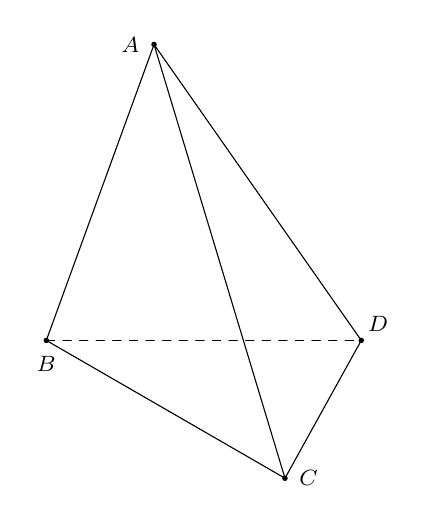
\begin{tikzpicture}[line join = round, line cap=round,>=stealth,font=\footnotesize,scale=1]
				\def\a{4} \def\b{4} \def\h{3.5}
				\path
				(0:0) coordinate (B)
				(70:\a) coordinate (A)
				(0:\b) coordinate (D)
				(-30:\h) coordinate (C)
				;
				\draw
				(A)--(B)--(C)--(D)--(A) (A)--(C)
				;
				\draw[dashed]
				(B) -- (D)
				;
				\foreach \x/\g in {A/180,C/0,B/-90,D/45}
				\fill (\x) circle (1pt)
				+(\g:3mm) node {$\x$};
			\end{tikzpicture}
		}
		\noindent
		Do đó
		$$V_{ABCD}=\dfrac{1}{6}\cdot 6\cdot 6\cdot 7\cdot \sqrt{1+2\cdot \dfrac{1}{9}\cdot \dfrac{1}{4}\cdot \dfrac{3}{7}-\left(\dfrac{1}{9}\right)^2 -\left(\dfrac{1}{4}\right)^2-\left(\dfrac{3}{7}\right)^2}.$$
		Ta có
		$$\cos (AB, CD)=\dfrac{\left|AC^2+BD^2-AD^2-BC^2\right|}{2AB\cdot CD}=\dfrac{7}{24}\Rightarrow \sin (AB, CD)=\dfrac{\sqrt{527}}{24}.$$
		Từ đó
		$$\mathrm{d}(AB, CD)=\dfrac{6V_{ABCD}}{AB\cdot CD\cdot \sin(AB,CD)}\approx 4{,}8.$$
	}
\end{ex}
\begin{ex}%[2D4V3-2]%[TDMZZ18]%[Nguyễn Đức Tuấn Anh]
	Cho tam giác đều $ABC$ có cạnh bằng $60$ cm. Ta thiết kế một bông hoa kì dị ba cánh được tạo thành từ ba đường parabol bằng nhau như hình vẽ. Mỗi đường có trục đối xứng trùng với đường cao của tam giác $ABC$ và tiếp xúc với hai cạnh của tam giác $ABC$. Hãy tính diện tích phần tô màu theo đơn vị cm$^2$ (\textit{không làm tròn ở các phép tính trung gian và làm tròn kết quả cuối cùng đến hàng đơn vị}).
	\begin{center}
		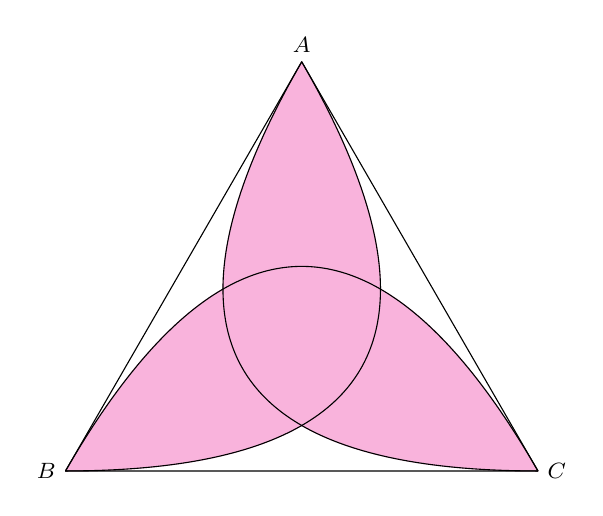
\begin{tikzpicture}[line cap=round, line join=round, >=stealth,font=\footnotesize]
			\pgfmathsetmacro{\sq}{sqrt(3)}
			\coordinate (A) at (0, 2*\sq);
			\coordinate (B) at (-3, -\sq);
			\coordinate (C) at (3, -\sq);
			\foreach \ang in {0, 120, 240} {
				\begin{scope}[rotate=\ang]
					\filldraw[magenta!30, draw=magenta!30] (0,0) -- plot[domain=-3:3, smooth, samples=100] (\x, {\sq/2 - \sq/6*(\x)^2}) -- cycle;
				\end{scope}
			}
			\foreach \ang in {0, 120, 240} {
				\begin{scope}[rotate=\ang]
					\draw plot[domain=-3:3, smooth, samples=100] (\x, {\sq/2 - \sq/6*(\x)^2});
				\end{scope}
			}
			\draw (A) -- (B) -- (C) -- cycle;
			\node[above] at (A) {$A$};
			\node[left] at (B) {$B$};
			\node[right] at (C) {$C$};
		\end{tikzpicture}
	\end{center}
	\par\shortans{1\,270}
	\loigiai{
		Chọn hệ trục tọa độ $Oxy$ như hình vẽ.
		\begin{center}
			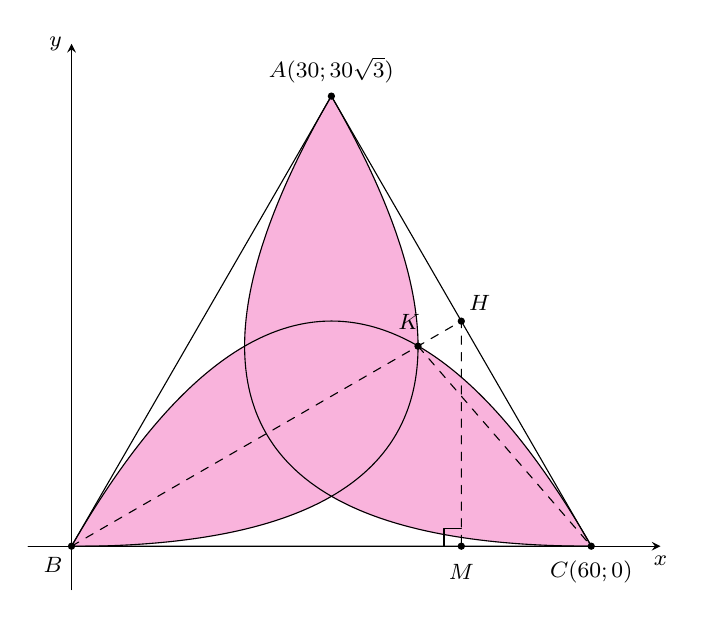
\begin{tikzpicture}[line cap=round, line join=round, >=stealth, scale=0.11, font=\footnotesize]
				\pgfmathsetmacro{\sq}{sqrt(3)}
				\path 
				(0, 0) coordinate (B)
				(60, 0) coordinate (C)
				(30, 30*\sq) coordinate (A)
				(30, 10*\sq) coordinate (G)
				(45, 15*\sq) coordinate (H)
				(45, 0) coordinate (M)
				(40, 40/\sq) coordinate (K);
				\foreach \ang in {0, 120, 240} {
					\begin{scope}[rotate around={\ang:(G)}]
						\filldraw[magenta!30, draw=magenta!30] (G) -- plot[domain=0:60, smooth, samples=100] (\x, {-\sq/60*(\x)^2 + \sq*\x}) -- cycle;
					\end{scope}
				}
				\foreach \ang in {0, 120, 240} {
					\begin{scope}[rotate around={\ang:(G)}]
						\draw plot[domain=0:60, smooth, samples=100] (\x, {-\sq/60*(\x)^2 + \sq*\x});
					\end{scope}
				}
				\draw[->] (-5, 0) -- (68, 0) node[below] {$x$};
				\draw[->] (0, -5) -- (0, 58) node[left] {$y$};
				\draw (A) -- (B) -- (C) -- cycle;
				\draw[dashed] (B) -- (H) -- (M) (K)--(C);
				\draw (45, 2) -- (43, 2) -- (43, 0); 
				\foreach \p/\lbl/\angle in {
					A/{A(30; 30\sqrt{3})}/90,
					B/{B}/225,
					C/{C(60; 0)}/-90,
					H/{H}/45,
					M/{M}/-90,
					K/K/110
				} {
					\fill (\p) circle (12pt);
					\path (\p) ++(\angle:3) node {$\lbl$};
				}
			\end{tikzpicture}
		\end{center}
		Do tam giác $ABC$ đều cạnh bằng $60$ nên đường cao tương ứng là $60 \cdot \dfrac{\sqrt{3}}{2} = 30\sqrt{3}$, suy ra $A\left(30; 30\sqrt{3}\right)$.\\
		Đường thẳng $AB$ đi qua gốc tọa độ và có hệ số góc $k = \tan 60^\circ = \sqrt{3}$ nên có phương trình $y = g(x) = \sqrt{3}x$.\\
		Xét đường parabol $(P)$ tương ứng với cánh hoa phía dưới cùng. Do tính đối xứng, $(P)$ đi qua $B(0;0)$ và $C(60;0)$. Theo giả thiết, $(P)$ tiếp xúc với cạnh $AB$ tại $B$.\\
		Giả sử phương trình của $(P)$ là $y = f(x) = ax^2 + bx + c$.\\
		Ta có hệ điều kiện
		\[
		\heva{&f(0) = 0 \\ &f(60) = 0 \\ &f'(0) = g'(0)} \Leftrightarrow \heva{&c = 0 \\ &60^2a + 60b = 0 \\ &b = \sqrt{3}} \Leftrightarrow \heva{&a = -\dfrac{\sqrt{3}}{60} \\ &b = \sqrt{3} \\ &c = 0.}
		\]
		Vậy phương trình của $(P)$ là $f(x) = -\dfrac{\sqrt{3}}{60}x^2 + \sqrt{3}x$.\\
		Từ hình vẽ, phần diện tích không tô màu gồm $6$ mảnh nhỏ bằng nhau (mỗi mảnh nằm trong một nửa của một tam giác tạo bởi đường cao và cạnh tam giác đều).\\
		Xét tam giác $BHC$ với $H$ là trung điểm của $AC$. Ta có $H\left(\dfrac{30+60}{2}; \dfrac{30\sqrt{3}+0}{2}\right) \Rightarrow H\left(45; 15\sqrt{3}\right)$.\\
		Gọi $S_0$ là diện tích phần không tô màu nằm trong tam giác $KHC$. \\
		Đường thẳng $BH$ đi qua $B(0;0)$ và $H(45; 15\sqrt{3})$ nên có phương trình $y = \dfrac{15\sqrt{3}}{45}x = \dfrac{1}{\sqrt{3}}x$.\\
		Hoành độ giao điểm $K$ của $BH$ và $(P)$ là nghiệm của phương trình
		\[
		-\dfrac{\sqrt{3}}{60}x^2 + \sqrt{3}x = \dfrac{1}{\sqrt{3}}x \Leftrightarrow -\dfrac{1}{60}x^2 + \dfrac{2}{3}x = 0 \Leftrightarrow \hoac{&x = 0 \\ &x = 40.}
		\]
		Ta lấy hoành độ $x_K = 40$.\\
		Gọi $M$ là hình chiếu vuông góc của $H$ lên trục $Ox$, ta có $M(45; 0)$.\\
		Diện tích tam giác vuông $HCM$ là $S_{\triangle HCM} = \dfrac{1}{2}HM \cdot MC = \dfrac{1}{2} \cdot 15\sqrt{3} \cdot 15 = \dfrac{225\sqrt{3}}{2}$.\\
		Diện tích $S_0$ được tính bằng
		\[
		S_0 = \displaystyle\int\limits_{40}^{45} \left(\dfrac{1}{\sqrt{3}}x - f(x)\right)\mathrm{\,d}x + \left( S_{\triangle HCM} - \displaystyle\int\limits_{45}^{60} f(x)\mathrm{\,d}x \right).
		\]
		Ta có
		\begin{itemize}
			\item $\displaystyle\int\limits_{40}^{45} \left(\dfrac{1}{\sqrt{3}}x - \left(-\dfrac{\sqrt{3}}{60}x^2 + \sqrt{3}x\right)\right)\mathrm{\,d}x  = \dfrac{325\sqrt{3}}{36}$.
			\item $\displaystyle\int\limits_{45}^{60} \left(-\dfrac{\sqrt{3}}{60}x^2 + \sqrt{3}x\right)\mathrm{\,d}x = \dfrac{375\sqrt{3}}{4}$.
		\end{itemize}
		Suy ra $S_0 = \dfrac{325\sqrt{3}}{36} + \dfrac{225\sqrt{3}}{2} - \dfrac{375\sqrt{3}}{4} = \dfrac{250\sqrt{3}}{9}$.\\
		Diện tích phần tô màu của bông hoa là
		\[
		S = S_{\triangle ABC} - 6S_0 = \dfrac{60^2\sqrt{3}}{4} - 6 \cdot \dfrac{250\sqrt{3}}{9}  \approx 1\,270\,\left(\text{cm}^2\right).
		\]
	}
\end{ex}
\begin{ex}%[2H5C2-7]%[TDMZZ18]%[Trương Tường]
	Trong không gian $Oxyz$ có đơn vị dài trên mỗi trục là centimet và có mặt đất là mặt phẳng $(Oxy)$, có một quả cầu $(S)$ có tâm cách mặt đất một đoạn bằng $180\text{ cm}$ và có bán kính bằng $80$ cm. Người ta muốn dùng ba sợi dây không giãn, mỗi sợi dây có một đầu buộc vào mặt đất và đầu còn lại buộc vào các điểm $A$, $B$, $C$ nằm trên mặt cầu $(S)$, sao cho cả ba sợi dây song song với giá của vectơ $\vec{u}=(1;2;3)$ và tam giác $ABC$ vuông cân với cạnh góc vuông bằng $60$ cm. Hãy tính theo đơn vị centimet giá trị nhỏ nhất của tổng độ dài $3$ đoạn dây này (không làm tròn ở các phép tính trung gian và làm tròn kết quả cuối cùng đến hàng đơn vị)?
	\begin{center}
		\begin{tikzpicture}[scale=0.35, >=stealth, line join=round, line cap=round, font=\scriptsize]
			\def\a{4}
			\def\b{1.25}
			\def\g{10} % góc quay
			\def\G{-10} % góc xác định tiếp điểm
			\pgfmathsetmacro{\ux}{-\a*sin(\G)*cos(\g)-\b*cos(\G)*sin(\g)}
			\pgfmathsetmacro{\uy}{-\a*sin(\G)*sin(\g)+\b*cos(\G)*cos(\g)}
			\path (0,0) coordinate (J)
			\foreach \l/\ang in {A1/0, A2/180, B1/90, B2/270, M/{\G}, C/50, A/-40, B/-130}{
				({\a*cos(\ang)*cos(\g)-\b*sin(\ang)*sin(\g)},{\a*cos(\ang)*sin(\g)+\b*sin(\ang)*cos(\g)}) coordinate (\l)
			}
			(M)+(\ux,\uy) coordinate (M1)
			($(M)!1!90:(M1)$) coordinate (M')
			(intersection of B1--B2 and M--M') coordinate (I)
			++(-90:8) coordinate (O)
			(O)+(10:6) coordinate (x)
			+(-20:6) coordinate (y)
			($(O)!-1!(x)$) coordinate (x')
			($(O)!-1!(y)$) coordinate (y')
			(O)++(-7.5,.5) coordinate (U)
			++(70:7) coordinate (U')
			(A)++(-110:5) coordinate (A')
			(B)++(-110:4) coordinate (B')
			(C)++(-110:5.5) coordinate (C')
			;
			%
			\fill [gray!40, opacity=.8] ($(x)+(y')-(O)$)--($(y')+(x')-(O)$)--($(x')+(y)-(O)$)--($(y)+(x)-(O)$)--cycle;
			\draw [fill=gray, opacity=.8, dash pattern=on 1.5pt off 1.5pt] (A)--(B)--(C)--cycle;
			\draw [->] (O)--($(I)+(90:6.5)$) node [left] {$z$};
			\draw [->] (O)--(x) node [above] {$x$};
			\draw [->] (O)--(y) node [right] {$y$};
			\draw [->] (U)--(U') node [left] {$\overrightarrow{u}=(1;2;3)$};
			\draw [dash pattern=on 1.5pt off 1.5pt] (A)--(A') (B)--(B') (C)--(C');
			\draw [samples=100, smooth, dash pattern=on 1.5pt off 1.5pt] plot [domain={\G}:{180-\G}] ({\a*cos(\x)*cos(\g)-\b*sin(\x)*sin(\g)},{\a*cos(\x)*sin(\g)+\b*sin(\x)*cos(\g)});
			\draw [gray, ball color=cyan, opacity=.8]
			(I) let \p1=($(M)-(I)$) in circle ({veclen(\p1)})
			;
			\draw [samples=100, smooth] plot [domain={-\G-180}:{\G}] ({\a*cos(\x)*cos(\g)-\b*sin(\x)*sin(\g)},{\a*cos(\x)*sin(\g)+\b*sin(\x)*cos(\g)});
			\draw [fill=black] (I) circle (1pt) node [left] {$I(0;0;180)$};
			\foreach \x in {A',B',C'}{
				\draw [fill=black] (\x) circle (1pt);
			}
			\foreach \x/\y in {O/-135, B/-70, A/-70, C/90}{
				\draw [fill=black] (\x) circle (1pt) ++(\y:0.6) node {$\x$};
			}
		\end{tikzpicture}
	\end{center}
	\par\shortans[oly]{$414$}
	\loigiai{
		\begin{center}
			\begin{tikzpicture}[scale=0.35, >=stealth, line join=round, line cap=round, font=\scriptsize]
				\def\a{4}
				\def\b{1.25}
				\def\g{10} % góc quay
				\def\G{-10} % góc xác định tiếp điểm
				\pgfmathsetmacro{\ux}{-\a*sin(\G)*cos(\g)-\b*cos(\G)*sin(\g)}
				\pgfmathsetmacro{\uy}{-\a*sin(\G)*sin(\g)+\b*cos(\G)*cos(\g)}
				\path (0,0) coordinate (J)
				\foreach \l/\ang in {A1/0, A2/180, B1/90, B2/270, M/{\G}, C/50, A/-40, B/-130}{
					({\a*cos(\ang)*cos(\g)-\b*sin(\ang)*sin(\g)},{\a*cos(\ang)*sin(\g)+\b*sin(\ang)*cos(\g)}) coordinate (\l)
				}
				(M)+(\ux,\uy) coordinate (M1)
				($(M)!1!90:(M1)$) coordinate (M')
				(intersection of B1--B2 and M--M') coordinate (I)
				++(-90:8) coordinate (O)
				(O)+(10:6) coordinate (x)
				+(-20:6) coordinate (y)
				($(O)!-1!(x)$) coordinate (x')
				($(O)!-1!(y)$) coordinate (y')
				(O)++(-7.5,.5) coordinate (U)
				++(70:7) coordinate (U')
				(U')+(-90:6.5) coordinate (U1)
				(A)++(-110:5) coordinate (A')
				(B)++(-110:4) coordinate (B')
				(C)++(-110:5.5) coordinate (C')
				($(A)!2/3!(J)$) coordinate (G)
				($(B')!.5!(C')$) coordinate (J')
				($(A')!2/3!(J')$) coordinate (G')
				;
				\fill [gray!40, opacity=.8] ($(x)+(y')-(O)$)--($(y')+(x')-(O)$)--($(x')+(y)-(O)$)--($(y)+(x)-(O)$)--cycle;
				\pic [draw, angle radius=0.1cm] {right angle=U'--U1--U};
				\pic [draw, "$\alpha$", angle radius=0.2cm, angle eccentricity=1.5] {angle=U1--U--U'};
				\draw [fill=gray, opacity=.8, dash pattern=on 1.5pt off 1.5pt] (A)--(B)--(C)--cycle;
				\draw [->] (O)--($(I)+(90:6.5)$) node [left] {$z$};
				\draw [->] (O)--(x) node [above] {$x$};
				\draw [->] (O)--(y) node [right] {$y$};
				\draw [->] (U)--(U') node [left] {$\overrightarrow{u}=(1;2;3)$};
				\draw [dash pattern=on 1.5pt off 1.5pt] (A)--(A') (B)--(B') (C)--(C') (G)--(G') (A)--(J) (J')--(A') (U)--(U1)--(U');
				\draw [samples=100, smooth, dash pattern=on 1.5pt off 1.5pt] plot [domain={\G}:{180-\G}] ({\a*cos(\x)*cos(\g)-\b*sin(\x)*sin(\g)},{\a*cos(\x)*sin(\g)+\b*sin(\x)*cos(\g)});
				\draw [semithick]
				(I) let \p1=($(M)-(I)$) in circle ({veclen(\p1)})
				;
				\draw [samples=100, smooth] plot [domain={-\G-180}:{\G}] ({\a*cos(\x)*cos(\g)-\b*sin(\x)*sin(\g)},{\a*cos(\x)*sin(\g)+\b*sin(\x)*cos(\g)});
				\draw (A')--(B')--(C')--cycle;
				\draw [fill=black] (I) circle (1pt) node [left] {$I(0;0;180)$};
				\foreach \x in {A',B',C'}{
					\draw [fill=black] (\x) circle (1pt);
				}
				\foreach \x/\y in {O/-135, B/90, A/75, C/90, A'/-10, B'/-90, C'/5, J/90, G/60, G'/25, J'/90}{
					\draw [fill=black] (\x) circle (1pt) ++(\y:0.6) node {$\x$};
				}
			\end{tikzpicture}
			\begin{tikzpicture}[scale=0.35, >=stealth, line join=round, line cap=round, font=\scriptsize]
				\def\a{4}
				\def\b{1.25}
				\def\g{15} % góc quay
				\def\G{-10} % góc xác định tiếp điểm
				\pgfmathsetmacro{\ux}{-\a*sin(\G)*cos(\g)-\b*cos(\G)*sin(\g)}
				\pgfmathsetmacro{\uy}{-\a*sin(\G)*sin(\g)+\b*cos(\G)*cos(\g)}
				\path (0,0) coordinate (J)
				\foreach \l/\ang in {A1/0, A2/180, B1/90, B2/270, M/{\G}, C/50, A/-40, B/-130}{
					({\a*cos(\ang)*cos(\g)-\b*sin(\ang)*sin(\g)},{\a*cos(\ang)*sin(\g)+\b*sin(\ang)*cos(\g)}) coordinate (\l)
				}
				(M)+(\ux,\uy) coordinate (M1)
				($(M)!1!90:(M1)$) coordinate (M')
				(intersection of B1--B2 and M--M') coordinate (I)
				++(-90:8) coordinate (O)
				(O)+(10:6) coordinate (x)
				+(-20:6) coordinate (y)
				($(O)!-1!(x)$) coordinate (x')
				($(O)!-1!(y)$) coordinate (y')
				(O)++(-7.5,.5) coordinate (U)
				++(70:7) coordinate (U')
				(U')+(-90:6.5) coordinate (U1)
				(A)++(-110:5) coordinate (A')
				(B)++(-110:4) coordinate (B')
				(C)++(-110:5.5) coordinate (C')
				($(A)!2/3!(J)$) coordinate (G)
				($(A')!2/3!(J')$) coordinate (G')
				++($(U1)-(U)$) coordinate (G1)
				(intersection cs: first line={(G)--($(G)+(U1)-(U')$)}, second line={(G')--(G1)}) coordinate (H)
				;
				\fill [gray!40, opacity=.8] ($(x)+(y')-(O)$)--($(y')+(x')-(O)$)--($(x')+(y)-(O)$)--($(y)+(x)-(O)$)--cycle;
				\pic [draw, angle radius=0.1cm] {right angle=U'--U1--U};
				\pic [draw, angle radius=0.1cm] {right angle=G--H--G'};
				\pic [draw, "$\alpha$", angle radius=0.2cm, angle eccentricity=1.5] {angle=U1--U--U'};
				\pic [draw, "$\alpha$", angle radius=0.2cm, angle eccentricity=1.5] {angle=H--G'--G};
				\draw [dash pattern=on 1.5pt off 1.5pt] (U)--(U1)--(U') (G)--(G') (G)--(H)--(G');
				\draw [->] (U)--(U') node [left] {$\overrightarrow{u}=(1;2;3)$};
				\foreach \x/\y in {G/60, G'/-90, H/-90}{
					\draw [fill=black] (\x) circle (1pt) ++(\y:0.6) node {$\x$};
				}
			\end{tikzpicture}
			\begin{tikzpicture}[scale=0.35, >=stealth, line join=round, line cap=round, font=\scriptsize]
				\def\a{4}
				\def\b{1.25}
				\def\g{10} % góc quay
				\def\G{-10} % góc xác định tiếp điểm
				\pgfmathsetmacro{\ux}{-\a*sin(\G)*cos(\g)-\b*cos(\G)*sin(\g)}
				\pgfmathsetmacro{\uy}{-\a*sin(\G)*sin(\g)+\b*cos(\G)*cos(\g)}
				\path (0,0) coordinate (J)
				\foreach \l/\ang in {A1/0, A2/180, B1/90, B2/270, M/{\G}, C/50, A/-40, B/-130}{
					({\a*cos(\ang)*cos(\g)-\b*sin(\ang)*sin(\g)},{\a*cos(\ang)*sin(\g)+\b*sin(\ang)*cos(\g)}) coordinate (\l)
				}
				(M)+(\ux,\uy) coordinate (M1)
				($(M)!1!90:(M1)$) coordinate (M')
				(intersection of B1--B2 and M--M') coordinate (I)
				++(-90:8) coordinate (O)
				(O)+(10:6) coordinate (x)
				+(-20:6) coordinate (y)
				($(O)!-1!(x)$) coordinate (x')
				($(O)!-1!(y)$) coordinate (y')
				($(A)!2/3!(J)$) coordinate (G)
				;
				%
				\pic [draw, angle radius=0.08cm] {right angle=I--J--B};
				\pic [draw, angle radius=0.08cm] {right angle=A--J--I};
				\fill [gray!40, opacity=.8] ($(x)+(y')-(O)$)--($(y')+(x')-(O)$)--($(x')+(y)-(O)$)--($(y)+(x)-(O)$)--cycle;
				\draw [fill=gray, opacity=.8, dash pattern=on 1.5pt off 1.5pt] (A)--(B)--(C)--cycle;
				\draw [dash pattern=on 1.5pt off 1.5pt] (I)--(J)--(A) (I)--(B) (I)--(G);
				\draw [->] (O)--($(I)+(90:6.5)$) node [left] {$z$};
				\draw [->] (O)--(x) node [above] {$x$};
				\draw [->] (O)--(y) node [right] {$y$};
				\draw [samples=100, smooth, dash pattern=on 1.5pt off 1.5pt] plot [domain={\G}:{180-\G}] ({\a*cos(\x)*cos(\g)-\b*sin(\x)*sin(\g)},{\a*cos(\x)*sin(\g)+\b*sin(\x)*cos(\g)});
				\draw [semithick]
				(I) let \p1=($(M)-(I)$) in circle ({veclen(\p1)})
				;
				\draw [samples=100, smooth] plot [domain={-\G-180}:{\G}] ({\a*cos(\x)*cos(\g)-\b*sin(\x)*sin(\g)},{\a*cos(\x)*sin(\g)+\b*sin(\x)*cos(\g)});
				\foreach \x/\y in {O/-135, B/90, A/75, C/90, J/-85, G/50, I/180}{
					\draw [fill=black] (\x) circle (1pt) ++(\y:0.6) node {$\x$};
				}
			\end{tikzpicture}
			\begin{tikzpicture}[scale=0.35, >=stealth, line join=round, line cap=round, font=\scriptsize]
				\def\a{4}
				\def\b{1.25}
				\def\g{10} % góc quay
				\def\G{-10} % góc xác định tiếp điểm
				\pgfmathsetmacro{\ux}{-\a*sin(\G)*cos(\g)-\b*cos(\G)*sin(\g)}
				\pgfmathsetmacro{\uy}{-\a*sin(\G)*sin(\g)+\b*cos(\G)*cos(\g)}
				\path (0,0) coordinate (J)
				\foreach \l/\ang in {A1/0, A2/180, B1/90, B2/270, M/{\G}, C/50, A/-40, B/-130}{
					({\a*cos(\ang)*cos(\g)-\b*sin(\ang)*sin(\g)},{\a*cos(\ang)*sin(\g)+\b*sin(\ang)*cos(\g)}) coordinate (\l)
				}
				(M)+(\ux,\uy) coordinate (M1)
				($(M)!1!90:(M1)$) coordinate (M')
				(intersection of B1--B2 and M--M') coordinate (I)
				++(-90:8) coordinate (O)
				(O)+(10:6) coordinate (x)
				+(-20:6) coordinate (y)
				($(O)!-1!(x)$) coordinate (x')
				($(O)!-1!(y)$) coordinate (y')
				($(A)!2/3!(J)$) coordinate (G)
				(A)++(-110:5) coordinate (A')
				(B)++(-110:4) coordinate (B')
				(C)++(-110:5.5) coordinate (C')
				($(A)!2/3!(J)$) coordinate (G)
				($(A')!2/3!(J')$) coordinate (G')
				++($(U1)-(U)$) coordinate (G1)
				(intersection cs: first line={(G)--($(G)+(U1)-(U')$)}, second line={(G')--(G1)}) coordinate (H)
				;
				%
				\fill [gray!40, opacity=.8] ($(x)+(y')-(O)$)--($(y')+(x')-(O)$)--($(x')+(y)-(O)$)--($(y)+(x)-(O)$)--cycle;
				\pic [draw, angle radius=0.1cm] {right angle=H--O--I};
				\draw [ball color=white, opacity=.8, name path=c]
				(I) let \p1=($(G)-(I)$) in circle ({veclen(\p1)});
				\draw [dash pattern=on 1.5pt off 1.5pt] (I)--(G)--(H) (O)--(H) (I)--(H);
				\draw (H)++(90:.2)--++(0:.2)--++(-90:.1);
				\draw [->, name path=a] (O)--($(I)+(90:6.5)$) node [left] {$z$};
				\draw [->] (O)--(x) node [above] {$x$};
				\draw [->] (O)--(y) node [right] {$y$};
				\foreach \x/\y in {O/-135, G/-35, I/180, H/-90}{
					\draw [fill=black] (\x) circle (1pt) ++(\y:0.6) node {$\x$};
				}
				\path [name intersections={of=a and c, by={,G"}}];
				\draw [fill=white] (G") circle (1.5pt);
				\draw [<-] (G")--++(-130:.5)--++(180:3) node [left, align=center] {Vị trí của $G$ \\ để $GH$ nhỏ nhất};
			\end{tikzpicture}
		\end{center}
		Gọi ba đoạn dây là $AA'$, $BB'$, $CC'$; $G$, $G'$ lần lượt là trọng tâm tam giác $ABC$, $A'B'C'$. \\
		Gọi $\alpha$ là góc tạo bởi giá của $\overrightarrow{u}$ và $(Oxy)$. Ta có \\
		\[\sin\alpha=\left|\cos\left(\overrightarrow{u},\overrightarrow{k}\right)\right|=\dfrac{\left|1 \cdot 0+2 \cdot 0+3 \cdot 1\right|}{\sqrt{1^2+2^2+3^2} \cdot \sqrt{0^2+0^2+1^2}}=\dfrac{3\sqrt{14}}{14}.\]
		Ta có 
		\begin{eqnarray*}
			\overrightarrow{AA'}+\overrightarrow{BB'}+\overrightarrow{CC'} &=& \left(\overrightarrow{AG}+\overrightarrow{GG'}+\overrightarrow{G'A'}\right)+\left(\overrightarrow{BG}+\overrightarrow{GG'}+\overrightarrow{G'B'}\right)+\left(\overrightarrow{CG}+\overrightarrow{GG'}+\overrightarrow{G'C'}\right) \\
			&=& \left(\overrightarrow{AG}+\overrightarrow{BG}+\overrightarrow{CG}\right)+3\overrightarrow{GG'}+\left(\overrightarrow{G'A'}+\overrightarrow{G'B'}+\overrightarrow{G'C'}\right) \\
			&=& 3\overrightarrow{GG'}. 
		\end{eqnarray*}
		Do đó $\left|\overrightarrow{AA'}+\overrightarrow{BB'}+\overrightarrow{CC'}\right|=3GG'$. \\
		Mà $\overrightarrow{AA'}$, $\overrightarrow{BB'}$, $\overrightarrow{CC'}$ cùng hướng nên $\left|\overrightarrow{AA'}+\overrightarrow{BB'}+\overrightarrow{CC'}\right|=AA'+BB'+CC'$. \\
		Suy ra $AA'+BB'+CC'=3GG'$. \\
		Như vậy $AA'+BB'+CC'$ đạt giá trị nhỏ nhất khi $GG'$ nhỏ nhất. \\
		Gọi $H$ là hình chiếu vuông góc của $G$ trên mặt phẳng $(Oxy)$. Khi đó 
		\[\sin\alpha=\dfrac{GH}{GG'} \Leftrightarrow GG'=\dfrac{GH}{\sin\alpha}=\dfrac{\sqrt{14} \cdot GH}{3}.\]
		Do đó $GG'$ nhỏ nhất khi $GH$ nhỏ nhất. \\
		Gọi $I$ là tâm mặt cầu $(S)$; $J$ là trung điểm của $BC$. Tam giác $ABC$ vuông tại $A$ nên $J$ là tâm đường tròn ngoại tiếp tam giác $ABC$. \\
		$\Rightarrow$ $IJ \perp (ABC)$.\\
		$\Rightarrow$ $IJ \perp JB$ và $IJ \perp JG$. \\
		$\Rightarrow$ $\triangle IJB$ và $\triangle IJG$ vuông tại $J$. \\
		Lại có $IB=80$, $BC=AB\sqrt{2}=60\sqrt{2}$, $JB=JC=JA=\dfrac{BC}{2}=30\sqrt{2}$. \\
		$\Rightarrow JG=\dfrac{1}{3}JA=10\sqrt{2}$, $IJ=\sqrt{IB^2-JB^2}=\sqrt{80^2-(30\sqrt{2})^2}=10\sqrt{46}$. \\
		Do đó $IG=\sqrt{IJ^2+JG^2}=\sqrt{(10\sqrt{46})^2+(10\sqrt{2})^2}=40\sqrt{3}$. \\
		Với ba điểm $I$, $G$, $H$ ta có $GH \ge IH-IG$. \\
		Mà $IH \ge IO$ nên $GH \ge IO-IG=180-40\sqrt{3}$. \\
		Dấu \lq\lq $=$\rq\rq~ xảy ra khi $H$ trùng $O$ đồng thời $I$, $G$, $H$ thẳng hàng và $G$ nằm giữa $I$ và $H$. \\
		$\Rightarrow$ $GH$ đạt giá trị nhỏ nhất bằng $180-40\sqrt{3}$. \\
		$\Rightarrow$ $GG'$ đạt giá trị nhỏ nhất bằng $\dfrac{\sqrt{14}\left(180-40\sqrt{3}\right)}{3}$. \\
		Vậy giá trị nhỏ nhất của tổng độ dài ba đoạn dây là $3 \cdot \dfrac{\sqrt{14}\left(180-40\sqrt{3}\right)}{3} \approx 414$ (cm).
	}
\end{ex}
\begin{ex}%[0D0C2-9]%[TDMZZ18-22-TLN]%[Nguyễn Văn Sang]
	Có $8$ viên bi màu đỏ được đánh số từ $1$ đến $8$, $5$ viên bi màu xanh được đánh số từ $1$ đến $5$, $3$ viên bi màu đen được đánh số từ $1$ đến $3$. Tiến hành xếp ngẫu nhiên $16$ viên bi này thành một hàng ngang. Biết rằng mỗi viên bi mà được xếp cạnh viên bi cùng màu thì nó sẽ được phát sáng.
	\begin{center}
		
\begin{tikzpicture}[scale=0.6, >=stealth, font=\sffamily\bfseries]
			% Bi đỏ
			\foreach \x in {1, ..., 8} {
				\fill[red, opacity=0.15] (\x, 0) circle (0.6);
				\fill[red, opacity=0.3] (\x, 0) circle (0.5);
				\shade[ball color=red!90] (\x, 0) circle (0.4);
				\node[white] at (\x, 0) {\x};
			}
			% Bi xanh
			\foreach \x in {1, ..., 5} {
				\shade[ball color=blue!90] (\x+8.5, 0) circle (0.4);
				\node[white] at (\x+8.5, 0) {\x};
			}
			% Bi đen
			\foreach \x in {1, ..., 3} {
				\shade[ball color=black!80] (\x+14, 0) circle (0.4);
				\node[white] at (\x+14, 0) {\x};
			}
		\end{tikzpicture}
	\end{center}
	Gọi $p$ là xác suất để có đúng $2$ viên bi được phát sáng. Hãy tính $10^6 p$ \textit{(không làm tròn ở các phép tính trung gian và làm tròn kết quả cuối cùng đến hàng đơn vị)}?
	\par\shortans[0]{8159}
	\loigiai{
		\textbf{Trường hợp 1: Cặp đôi phát sáng là màu Đỏ (Đỏ - Đỏ)}
		\begin{itemize}
			\item \textbf{Chọn bi:} Chọn 2 viên Đỏ trong 8 viên để làm khối đôi: $\mathrm{C}_{8}^{2} = 28$ cách.
			\item \textbf{Gộp khối:} Ta còn lại: $7$ khối Đỏ (1 đôi + 6 đơn) và $8$ khối còn lại (gồm 5 khối Xanh, 3 khối Đen).
			\item \textbf{Nguyên lý xếp màu sắc cốt lõi:}
			\begin{itemize}
				\item Xếp 8 khối Xanh và Đen thành hàng trước $\Rightarrow$ có $\mathrm{C}_{8}^{3} = 56$ cách xếp màu sắc.
				\item Hàng 8 khối này tạo ra đúng \textbf{9 khoảng trống} (7 khe giữa và 2 đầu mút).
				\item Gọi $m$ là số cặp cùng màu đứng cạnh nhau sẵn trong hàng Xanh và Đen. Khi đó, $m$ vị trí trùng màu này \textbf{bắt buộc phải nhận 1 khối Đỏ} để chia cắt chúng ra.
				\item Như vậy, ta đã dùng mất $m$ khối Đỏ vào $m$ vị trí bắt buộc. Ta còn lại $7-m$ khối Đỏ tự do để xếp vào $9-m$ khoảng trống còn lại. Số cách chọn vị trí cho các khối Đỏ còn lại này là: $\mathrm{C}_{9-m}^{7-m} = \mathrm{C}_{9-m}^{2}$ cách.
			\end{itemize}
		\end{itemize}
		\textbf{6 khả năng xảy ra của biến số $m$:}
		\begin{itemize}
			\item \textbf{Khả năng 1 ($m=6$): Có 2 dãy Xanh và Đen bị trùng nhau hoàn toàn (VD: X-X-X-X-X-Đ-Đ-Đ)}
			\\ Có 6 khe trùng màu bắt buộc phải nhét Đỏ. Số cách chọn chỗ cho các khối Đỏ còn lại là $\mathrm{C}_{9-6}^{2} = \mathrm{C}_{3}^{2} = 3$ cách.
			\\ Tổng số cách phối màu: $2 \times 3 = \mathbf{6}$ cách.
			\begin{center}
				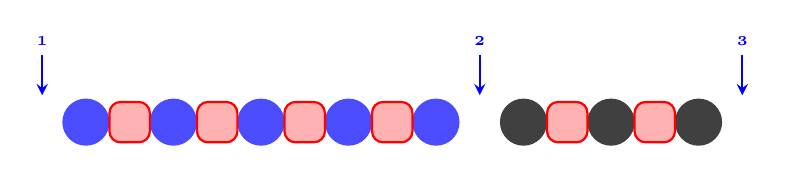
\begin{tikzpicture}[scale=0.855, >=stealth]
					\foreach \x / \col in {1/blue!70, 2/blue!70, 3/blue!70, 4/blue!70, 5/blue!70, 6/black!75, 7/black!75, 8/black!75} {
						\fill[\col] (\x*1.3, 0) circle (0.35);
					}
					\foreach \x in {1, 2, 3, 4, 6, 7} {
						\draw[fill=red!30, draw=red, thick, rounded corners] (\x*1.3+0.35, -0.3) rectangle ++(0.6, 0.6);
					}
					\foreach \x / \i in {0/1, 5/2, 8/3} {
						\draw[->, blue, thick] (\x*1.3+0.65, 1.0) -- (\x*1.3+0.65, 0.4);
						\node[blue, font=\tiny\bfseries] at (\x*1.3+0.65, 1.2) {\i};
					}
				\end{tikzpicture}
			\end{center}
			
			\item \textbf{Khả năng 2 ($m=5$): Có 6 dãy Xanh và Đen dính chùm ít hơn (VD: X-X-X-X-Đ-Đ-Đ-X)}
			\\ Có 5 khe trùng màu bắt buộc phải nhét Đỏ. Số cách chọn chỗ cho các khối Đỏ còn lại là $\mathrm{C}_{9-5}^{2} = \mathrm{C}_{4}^{2} = 6$ cách.
			\\ Tổng số cách phối màu: $6 \times 6 = \mathbf{36}$ cách.
			\begin{center}
				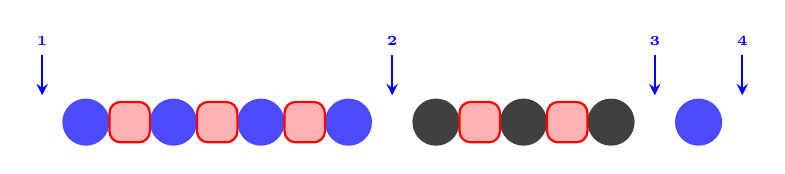
\begin{tikzpicture}[scale=0.855, >=stealth]
					\foreach \x / \col in {1/blue!70, 2/blue!70, 3/blue!70, 4/blue!70, 5/black!75, 6/black!75, 7/black!75, 8/blue!70} {
						\fill[\col] (\x*1.3, 0) circle (0.35);
					}
					\foreach \x in {1, 2, 3, 5, 6} {
						\draw[fill=red!30, draw=red, thick, rounded corners] (\x*1.3+0.35, -0.3) rectangle ++(0.6, 0.6);
					}
					\foreach \x / \i in {0/1, 4/2, 7/3, 8/4} {
						\draw[->, blue, thick] (\x*1.3+0.65, 1.0) -- (\x*1.3+0.65, 0.4);
						\node[blue, font=\tiny\bfseries] at (\x*1.3+0.65, 1.2) {\i};
					}
				\end{tikzpicture}
			\end{center}
			
			\item \textbf{Khả năng 3 ($m=4$): Có 16 dãy Xanh và Đen dính chùm vừa phải (VD: X-X-X-Đ-Đ-X-X-Đ)}
			\\ Có 4 khe trùng màu bắt buộc phải nhét Đỏ. Số cách chọn chỗ cho các khối Đỏ còn lại là $\mathrm{C}_{9-4}^{2} = \mathrm{C}_{5}^{2} = 10$ cách.
			\\ Tổng số cách phối màu: $16 \times 10 = \mathbf{160}$ cách.
			\begin{center}
				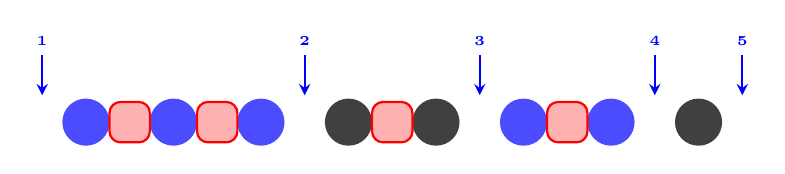
\begin{tikzpicture}[scale=0.855, >=stealth]
					\foreach \x / \col in {1/blue!70, 2/blue!70, 3/blue!70, 4/black!75, 5/black!75, 6/blue!70, 7/blue!70, 8/black!75} {
						\fill[\col] (\x*1.3, 0) circle (0.35);
					}
					\foreach \x in {1, 2, 4, 6} {
						\draw[fill=red!30, draw=red, thick, rounded corners] (\x*1.3+0.35, -0.3) rectangle ++(0.6, 0.6);
					}
					\foreach \x / \i in {0/1, 3/2, 5/3, 7/4, 8/5} {
						\draw[->, blue, thick] (\x*1.3+0.65, 1.0) -- (\x*1.3+0.65, 0.4);
						\node[blue, font=\tiny\bfseries] at (\x*1.3+0.65, 1.2) {\i};
					}
				\end{tikzpicture}
			\end{center}
			
			\item \textbf{Khả năng 4 ($m=3$): Có 16 dãy Xanh và Đen phân tán đều hơn (VD: X-X-Đ-X-X-Đ-Đ-X)}
			\\ Có 3 khe trùng màu bắt buộc phải nhét Đỏ. Số cách chọn chỗ cho các khối Đỏ còn lại là $\mathrm{C}_{9-3}^{2} = \mathrm{C}_{6}^{2} = 15$ cách.
			\\ Tổng số cách phối màu: $16 \times 15 = \mathbf{240}$ cách.
			\begin{center}
				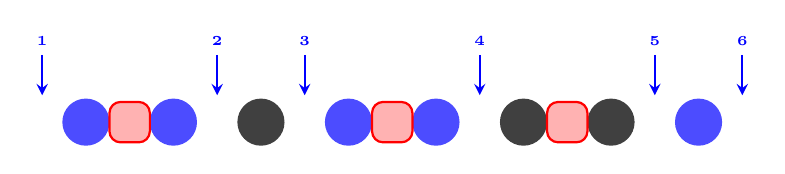
\begin{tikzpicture}[scale=0.855, >=stealth]
					\foreach \x / \col in {1/blue!70, 2/blue!70, 3/black!75, 4/blue!70, 5/blue!70, 6/black!75, 7/black!75, 8/blue!70} {
						\fill[\col] (\x*1.3, 0) circle (0.35);
					}
					\foreach \x in {1, 4, 6} {
						\draw[fill=red!30, draw=red, thick, rounded corners] (\x*1.3+0.35, -0.3) rectangle ++(0.6, 0.6);
					}
					\foreach \x / \i in {0/1, 2/2, 3/3, 5/4, 7/5, 8/6} {
						\draw[->, blue, thick] (\x*1.3+0.65, 1.0) -- (\x*1.3+0.65, 0.4);
						\node[blue, font=\tiny\bfseries] at (\x*1.3+0.65, 1.2) {\i};
					}
				\end{tikzpicture}
			\end{center}
			
			\item \textbf{Khả năng 5 ($m=2$): Có 12 dãy Xanh và Đen đan xen rất tốt (VD: X-X-Đ-X-Đ-X-X-Đ)}
			\\ Có 2 khe trùng màu bắt buộc phải nhét Đỏ. Số cách chọn chỗ cho các khối Đỏ còn lại là $\mathrm{C}_{9-2}^{2} = \mathrm{C}_{7}^{2} = 21$ cách.
			\\ Tổng số cách phối màu: $12 \times 21 = \mathbf{252}$ cách.
			\begin{center}
				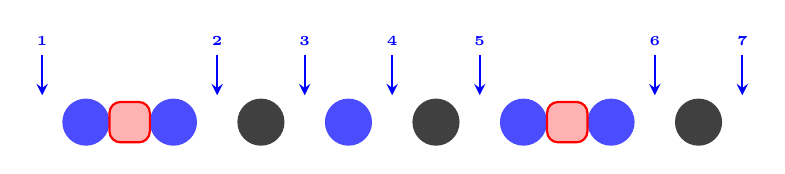
\begin{tikzpicture}[scale=0.855, >=stealth]
					\foreach \x / \col in {1/blue!70, 2/blue!70, 3/black!75, 4/blue!70, 5/black!75, 6/blue!70, 7/blue!70, 8/black!75} {
						\fill[\col] (\x*1.3, 0) circle (0.35);
					}
					\foreach \x in {1, 6} {
						\draw[fill=red!30, draw=red, thick, rounded corners] (\x*1.3+0.35, -0.3) rectangle ++(0.6, 0.6);
					}
					\foreach \x / \i in {0/1, 2/2, 3/3, 4/4, 5/5, 7/6, 8/7} {
						\draw[->, blue, thick] (\x*1.3+0.65, 1.0) -- (\x*1.3+0.65, 0.4);
						\node[blue, font=\tiny\bfseries] at (\x*1.3+0.65, 1.2) {\i};
					}
				\end{tikzpicture}
			\end{center}
			
			\item \textbf{Khả năng 6 ($m=1$): Có 4 dãy Xanh và Đen đan xen gần như hoàn hảo (VD: X-Đ-X-Đ-X-Đ-X-X)}
			\\ Chỉ có duy nhất 1 khe trùng màu bắt buộc nhét Đỏ. Số cách chọn chỗ cho các khối Đỏ còn lại là $\mathrm{C}_{9-1}^{2} = \mathrm{C}_{8}^{2} = 28$ cách.
			\\ Tổng số cách phối màu: $4 \times 28 = \mathbf{112}$ cách.
			\begin{center}
				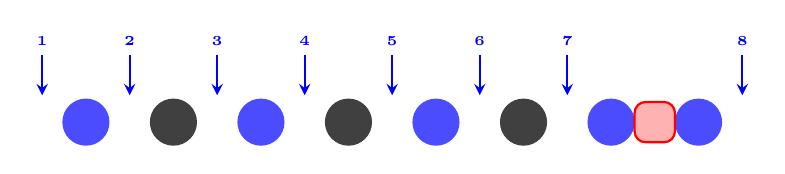
\begin{tikzpicture}[scale=0.855, >=stealth]
					\foreach \x / \col in {1/blue!70, 2/black!75, 3/blue!70, 4/black!75, 5/blue!70, 6/black!75, 7/blue!70, 8/blue!70} {
						\fill[\col] (\x*1.3, 0) circle (0.35);
					}
					\foreach \x in {7} {
						\draw[fill=red!30, draw=red, thick, rounded corners] (\x*1.3+0.35, -0.3) rectangle ++(0.6, 0.6);
					}
					\foreach \x / \i in {0/1, 1/2, 2/3, 3/4, 4/5, 5/6, 6/7, 8/8} {
						\draw[->, blue, thick] (\x*1.3+0.65, 1.0) -- (\x*1.3+0.65, 0.4);
						\node[blue, font=\tiny\bfseries] at (\x*1.3+0.65, 1.2) {\i};
					}
				\end{tikzpicture}
			\end{center}
		\end{itemize}
		
		\begin{itemize}
			\item[] $\Rightarrow$ Tổng số cách xếp mô hình màu sắc hợp lệ cho cả TH1 là: $6 + 36 + 160 + 240 + 252 + 112 = \mathbf{806}$ cách.
			\item Số cách xếp hoán vị thứ tự các viên bi cụ thể là: $7! \times 5! \times 3!$.
			\item Số cách xếp hoàn chỉnh cho TH1:
			\[ n_1 = 28 \times 806 \times (7! \times 5! \times 3!) = 5642 \times 8! \times 5! \times 3! \]
		\end{itemize}
		
		\vfill
		\textbf{Trường hợp 2: Cặp đôi phát sáng là màu Xanh (Xanh - Xanh)}
		\begin{itemize}
			\item \textbf{Chọn bi:} Chọn 2 viên Xanh trong 5 viên làm khối đôi: $\mathrm{C}_{5}^{2} = 10$ cách.
			\item \textbf{Gộp khối:} Ta còn lại: $8$ khối Đỏ và $7$ khối màu khác (gồm 4 khối Xanh, 3 khối Đen).
		\end{itemize}
		
		\begin{center}
			\begin{tikzpicture}[scale=0.97, >=stealth]
				% 8 khối đỏ
				\foreach \x in {1, ..., 8} {
					\draw[fill=red!20, draw=red, thick, rounded corners] (\x*1.5, 0) rectangle ++(0.7, 0.5);
					\node[red, font=\bfseries\small] at (\x*1.5+0.35, 0.25) {Đỏ};
				}
				% 7 vị trí trống xen kẽ bắt buộc phải điền đầy
				\foreach \x in {1, ..., 7} {
					\draw[fill=blue!10, draw=blue, thick, dashed, rounded corners] (\x*1.5+0.85, 0) rectangle ++(0.5, 0.5);
					\node[blue, font=\bfseries\small] at (\x*1.5+1.1, 0.25) {?};
				}
			\end{tikzpicture}
		\end{center}
		
		\begin{itemize}
			\item Vì có tới 8 khối Đỏ nhưng chỉ có 7 khối màu khác, để các khối Đỏ không chạm nhau thì toàn bộ 7 khối này bắt buộc phải xếp chính xác vào 7 khe trống ở giữa như hình vẽ. Lúc này, các khối màu khác đã bị cô lập hoàn toàn bởi các vách ngăn Đỏ nên xếp thế nào cũng không sợ trùng màu giữa chúng: $\mathrm{C}_{7}^{4} = 35$ cách xếp màu.
			\item Số cách xếp hoàn chỉnh cho TH2:
			\[ n_2 = 10 \times 35 \times (8! \times 4! \times 3!) = 175 \times 8! \times 5! \times 3! \]
		\end{itemize}
		
		\vfill
		\textbf{Trường hợp 3: Cặp đôi phát sáng là màu Đen (Đen - Đen)}
		\begin{itemize}
			\item \textbf{Chọn bi:} Chọn 2 viên Đen trong 3 viên làm khối đôi: $\mathrm{C}_{3}^{2} = 3$ cách.
			\item \textbf{Gộp khối:} Ta còn lại: $8$ khối Đỏ và $7$ khối màu khác (gồm 5 khối Xanh, 2 khối Đen).
		\end{itemize}
		
		\begin{center}
			\begin{tikzpicture}[scale=0.97, >=stealth]
				% Tương tự TH2
				\foreach \x in {1, ..., 8} {
					\draw[fill=red!20, draw=red, thick, rounded corners] (\x*1.5, 0) rectangle ++(0.7, 0.5);
					\node[red, font=\bfseries\small] at (\x*1.5+0.35, 0.25) {Đỏ};
				}
				\foreach \x in {1, ..., 7} {
					\draw[fill=black!10, draw=black, thick, dashed, rounded corners] (\x*1.5+0.85, 0) rectangle ++(0.5, 0.5);
					\node[black, font=\bfseries\small] at (\x*1.5+1.1, 0.25) {?};
				}
			\end{tikzpicture}
		\end{center}
		
		\begin{itemize}
			\item Tương tự Trường hợp 2, 7 khối màu khác bắt buộc phải nằm gọn vào 7 khe giữa của các khối Đỏ để ngăn chúng chạm nhau. Số cách xếp màu cho 5 khối Xanh và 2 khối Đen vào 7 chỗ này là: $\mathrm{C}_{7}^{5} = 21$ cách.
			\item Số cách xếp hoàn chỉnh cho TH3:
			\[ n_3 = 3 \times 21 \times (8! \times 5! \times 2!) = 63 \times 8! \times 5! \times 3! \]
		\end{itemize}
		
		\vfill
		\textbf{Bước 3: Kết luận xác suất}
		\begin{itemize}
			\item Tổng số kết quả thuận lợi cho biến cố
			\[ n(A) = n_1 + n_2 + n_3 = (5642 + 175 + 63) \times 8! \times 5! \times 3! = 5880 \times 8! \times 5! \times 3! \]
			\item Xác suất $p$ của biến cố là
			\[ p = \dfrac{5880 \times 8! \times 5! \times 3!}{16!} = \dfrac{7}{858} \]
			\item Giá trị biểu thức đề bài yêu cầu
			\[ 10^6 p = 10^6 \times \dfrac{7}{858} \approx 8159.\]
		\end{itemize}
	}
\end{ex}